\chapter{Solution}\label{chap:solution}

This chapter presents the solutions to the problems exposed previously. It explains the rationale behind them, as well as why they were preferred over their alternatives.

First, the general architecture is described, presenting the multiple components of the application. Afterward, each component is described in more detail, regarding its functionality and implementation.

\section{General Services Architecture}

This section describes the general architecture of the system. It is composed of multiple microservices, each handling a specific part of the problem. The main services are the ones dealing with the frontend application --- the web application itself ---, the conflict handling, and the user reputation\hyphenation{re-pu-ta-tion}. Additional services are built in order to achieve a functional whole, and they will be described below. Figure~\ref{fig:services-arch} shows the system architecture design and how the services connect to one another. Listing~\ref{lst:docker-compose-definition} contains all the configured services, including proxies and helper services.

All of these services are managed using Docker\footnote{https://www.docker.com/}. Each service is built within a Docker Container, allowing it to be easy deployed and replicated across machines for scalability and fault tolerance. It also ensures that every deployment is identical, no matter the host machine and environment it is deployed on.

Additionally, Docker Compose\footnote{https://docs.docker.com/compose/} is used to define how the different containers in a multi-container application should interact with each other, allowing us to start the application as one entity, instead of multiple isolated containers. It conveniently provides an internal DNS so that containers can reach each other by their service name. Listing~\ref{list:conflict-resolution-strategies-frontend} shows the configuration file for the different docker services. Each service has a unique name, e.g., \say{apacheproxy}, \say{frontend}, and fields configuring its deployment. The build property specifies the location of the Dockerfile associated with the service image; the ports are defined in \verb+<Host Port>:<Container Port>+ format, and map to which port on the host --- i.e., the machine that is running docker --- the services should listen. Additional properties such as \say{restart} configure the behavior on failure, and storage containers, such as the \say{couchdb} and \say{mongo}, are configured to have data volumes, so that when the container is shut down the data is preserved on the host machine, so that it can be recovered later when it restarts. The \say{depends\_on} property makes sure that the service on which some service depends, is running when the dependent service is running.

\lstset{float=H}

\begin{lstlisting}[label={lst:docker-compose-definition},caption={docker-compose.yml file --- Docker services definition}]
    version: '3.1'
    services:
        apacheproxy:
            build: apache-reverse-proxy/
            restart: always
            ports: 
                - "80:80"
        frontend: 
            build: .
            ports: 
                - "5000:80"
        apiproxy: 
            build: api/
            ports: 
                - "5001:80"
        conflicthandlerservice:
            build: conflict-handler-service/
            restart: always
            ports:
                - "5002:80"
            depends_on: 
                - couchdb
        reputationservice:
            build: reputation-service/
            restart: always
            ports:
                - "5003:80"
            depends_on: 
                - mongo
        couchdb:
            build: couchdb
            environment:
                - COUCHDB_USER=***
                - COUCHDB_PASSWORD=***
            ports:
                - "5984:5984"
            volumes: 
                - ./couchdb-data:/opt/couchdb/data
        mongo:
            image: mongo
            ports:
                - "27017:27017"
            volumes: 
                - ./mongodb-data:/data/db
\end{lstlisting}


Finally, a microservice architecture promotes isolation and independence of services, which in turn allows for easier development and testing. Different teams can work on each service, which has a single purpose, and they only need to agree on the interface and how they can communicate between them.


\begin{figure}[h]
    \begin{center}
        \leavevmode
        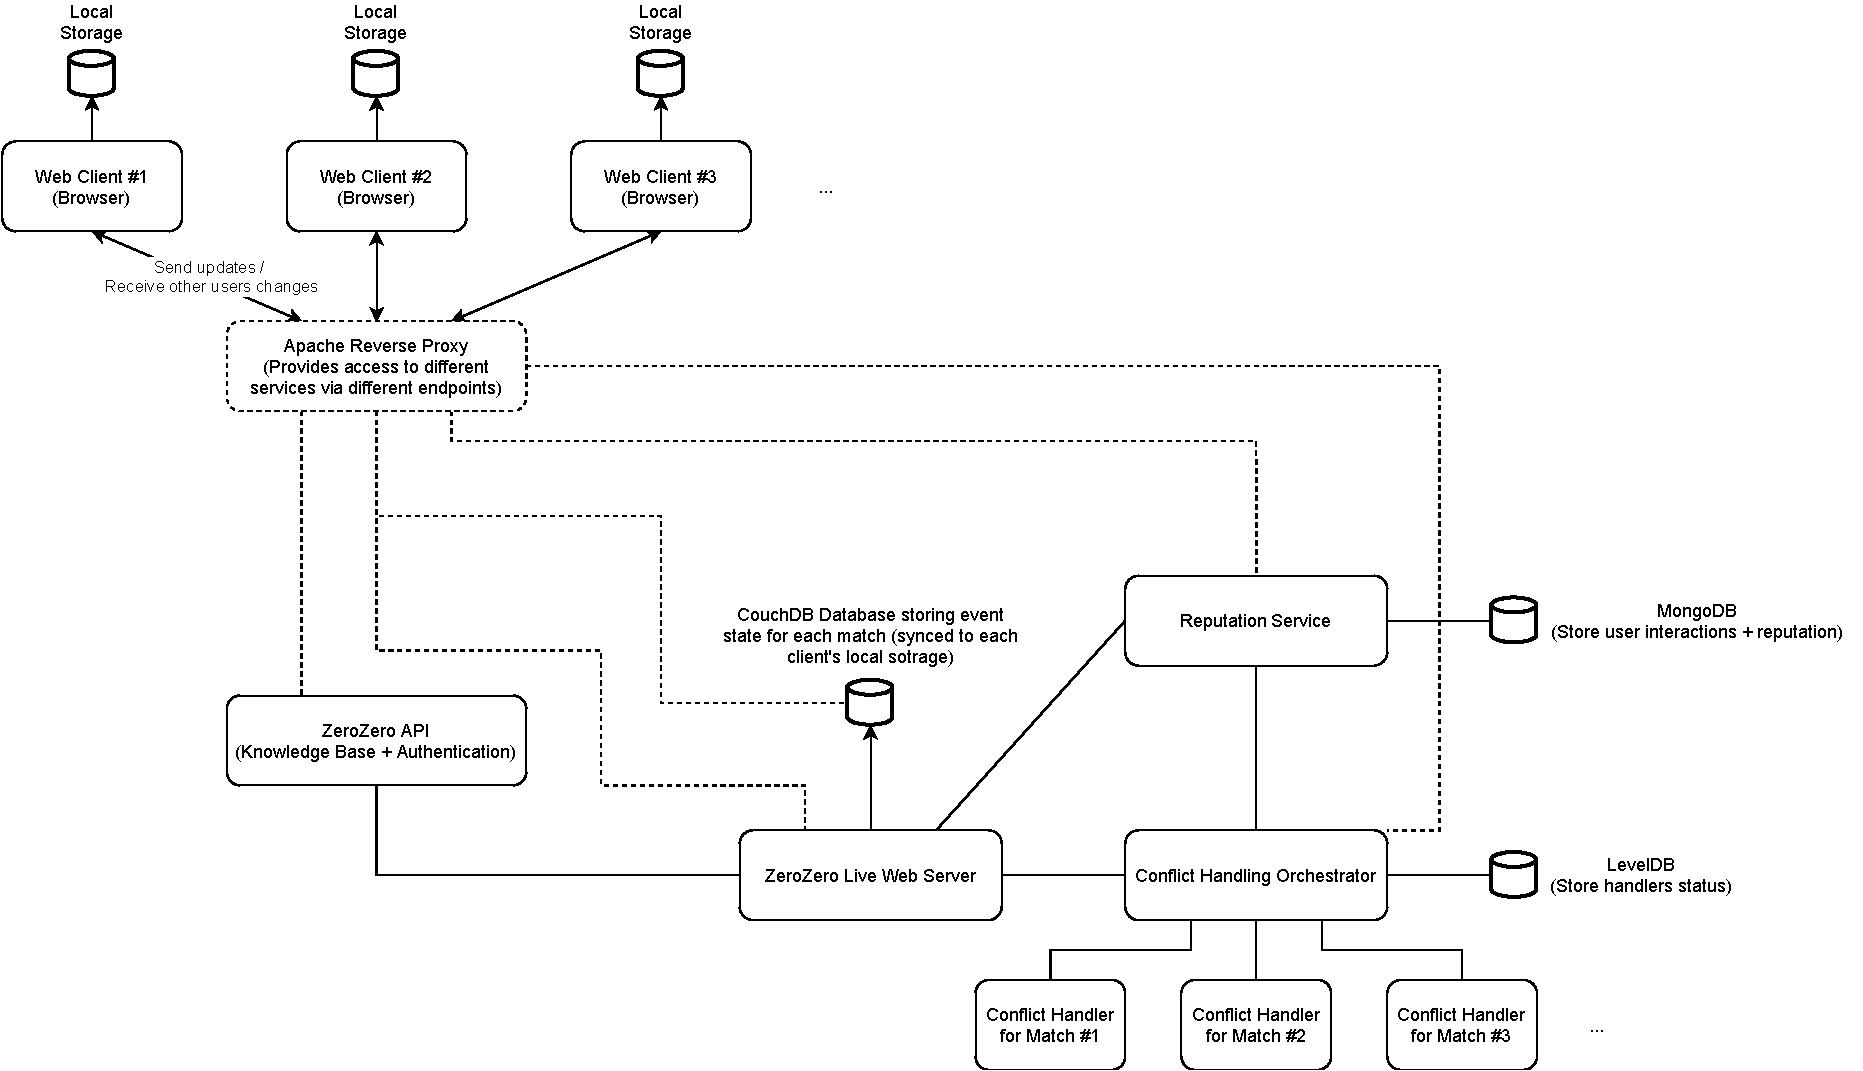
\includegraphics[width=\textwidth]{zerozerolive-arch.pdf}
        \caption{Architecture design of the zerozero.live system}
        \label{fig:services-arch}
    \end{center}
\end{figure}

\section{Reverse Proxy}

In the zerozero.live deployment, only the 443 --- HTTPS --- port is exposed to the internet, thus, to expose multiple services, it cannot be done in multiple ports, at least not from the outside. Due to this, a reverse proxy is required to map each service --- and its specific port --- to an endpoint on the main domain zerozero.live:
 
\begin{itemize}
    \item \textbf{/} Redirects to the client application --- the application's frontend;
    \item \textbf{/api} Redirects to a small proxy that communicates with the ZeroZero API;
    \item \textbf{/db} Redirects to the CouchDB, holding the match events in real time;
    \item \textbf{/manager} Redirects to the conflict handling services orchestrator, which monitors the conflict handlers for each match;
    \item \textbf{/reputation-manager} Redirects to the reputation service, which registers the interactions and calculates the reputation updates for users.
\end{itemize}

The following sections will dive deeper on the purpose and implementation details of each aforementioned service, which compose the whole application 

\section{CouchDB}

CouchDB is a document-oriented, multi-master database, which allows for easy replication between nodes. This enables data to flow seamlessly from web browsers to the database and vice versa, powering offline-first applications while being developer friendly, since the API that interacts with the local database --- powered by PouchDB --- is the same that interacts with the remote database --- CouchDB.

When compared to the previously analyzed alternatives, namely ShareDB and CRDT solutions such as Automerge, CouchDB is older and thus more \textit{battle tested} than the rest, while also having frequent releases --- the latest stable to date is from September, 2020. ShareDB has also been around for some time, since 2013, however, it offers a lower level alternative to conflict resolution using OT. It allows integration with any database and offers similar features to CouchDB, but I have found it difficult to program custom conflict resolution strategies, very much important to this work. From the three, Automerge is the youngest (2017), and it relies on a different approach to conflict resolution, based on CRDT. As it does not require a central server, it merges documents automatically and I could not find how to add custom resolution of conflicts, which led me to choose the CouchDB alternative.

It is based on documents which are JSON objects with at least an id and a revision identifier. CouchDB then uses this to detect conflicts --- if it has the same id, it may conflict --- and to resolve them. It works by creating a tree of documents, where the leaf nodes are the current winners, branches represent conflicting revisions, which are kept to be resolved by the application if needed. CouchDB will choose a winner automatically and deterministically, so that every client has the same version of the data. However it is possible to resolve the conflicts afterwards, by choosing a conflicting version as the winner, which appends a new node to the tree, after the previous winner, making the previously conflicting document the new leaf node, and thus the new winner for that document id.

Finally, this has the advantage of having a browser version, powered by PouchDB, which replicates the database to the browser's IndexedDB, and its API is the same as CouchDB's. This makes the application offline first, since all the changes are made to the local database, and continuously synchronized to the remote database.

\section{Conflict Handling}

Conflict handling is divided into two separate parts. One for the conflict handling of a single match, which is responsible to handle the conflicts themselves on the match level, and another for the orchestration of handlers themselves, which is responsible for the launching and orchestration of the match conflict handler processes. But first, it's important to set some concepts regarding conflict detection and documents' structure.

\subsection{Conflict Detection}

As events are introduced by users, conflicts may arise. The conflicting events are the ones whose documents share the same $\_id$. If we want documents to conflict, they cannot have unique ids, so the following structure was defined for each event $\_id$:
\begin{equation}
    eventMinute-eventMinuteExtra-eventCategory
\end{equation}

By having this structure, when any event from the same category is inserted, referring to the same game minute as another, they will conflict. Event categories are defined in such a way that events from different categories do not conflict. Some category examples include goal related events (\textit{Goal}, \textit{Own Goal}, \textit{Big Scoring Opportunity}, etc.), card related events (\textit{Yellow Card}, \textit{Red Card}), or time events (\textit{Start Whistle}, \textit{End of 1st Half}, \textit{Final Whistle}, etc.)

This will ensure that we have a basic conflict detection, however it can easily be noticed that even in the same category there may be events on the same minute: There can be a \textit{Big Scoring Opportunity} immediately followed by a \textit{Goal}, or even two \textit{Yellow Cards} for two different players, or even the same one which will wrongly conflict.

To improve the experience, a conflict handler is needed, in order to automatically solve conflicts as best as possible.

There are two concepts to understand going forward: events, and documents. Events are the instances of events, as used by the ZeroZero API, such as a \textit{Goal}, \textit{Own Goal}, or \textit{Big Scoring Opportunity}. These include the event type id, their category, some template text and a representative image to be rendered associated with it, among other fields. The complete list of events is present in Appendix~\ref{annex:api-events}. Documents is a wrapper on the API events, which are stored in the CouchDB database, and used on the ZeroZero Live exclusively. They are structured as follows:

\begin{description}
    \item[\_id] the document id, used to detect conflicts, as explained above;
    \item[\_rev] the document's revision, in order to provide the history level of the changes tree of this document $\_id$;
    \item[timestamp] a UNIX timestamp to help sorting the events that are generated for the same match minute;
    \item[id] the id of the corresponding event on the ZeroZero API, received on insert, and required to edit or delete this event from the API;
    \item[fk\_jogo] the match id;
    \item[equipa] the respective team's id;
    \item[fk\_user] id of the user that generated the event;    
    \item[fk\_jogador] id of the player the event refers to;    
    \item[fk\_jogador\_out] id of the secondary player the event refers to (used in the substitution event);    
    \item[minuto] the match minute;
    \item[minuto\_extra] the extra minute, in case the event happened during injury time;
    \item[texto] the event's text (after template interpolation)
    \item[event\_id] the event type id;    
    \item[fk\_live\_tpevent] the same as $event\_id$;
    \item[ignore\_minuto] 1 if the minute should be ignored, 0 otherwise;
    \item[categoria] the event's category;  
    \item[vodafone\_clock\_time] a timestamp indicating the video mark when the event can be visualized;
    \item[insert] flag indicating if the event should be inserted to the ZeroZero\hyphenation{ZeroZero} API;
    \item[synced\_from\_api] flag indicating if this document came from a synchronization from the ZeroZero API, instead of being inserted by a user manually. 
\end{description}

Regarding conflict resolution, the main fields to take into account are the $\_id$ and $\_rev$. A more detailed explanation is presented below on how these fields are used to detect and resolve conflicts between two documents.

\subsection{Conflict Handler}

As previously noted, the Conflict Handler will help resolve some existing conflict automatically, based on the conflicting events and the match context, in order to only rely on users to resolve pending conflicts as a last resource.

This is a Node.js process that will use PouchDB to connect to the remote CouchDB and listen for changes. It has two main responsibilities:
\begin{itemize}
    \item If the document does not have conflicts sync with ZeroZero API, by inserting, editing or deleting the event from their database, depending on the operation
    \item If the document has conflicts, try to resolve them according to the specified rules, by either deleting the conflict and keeping the current winner, deleting the conflict and adding it \textit{after} the previous winner, to choose it as winner, or keeping both documents, by deleting the conflict and adding a replicated document with a unique suffix added to the id so that it won't conflict again (See Figure~\ref{graph:keep-both-resolution}).
\end{itemize}

\begin{figure}[h]
    \centering
    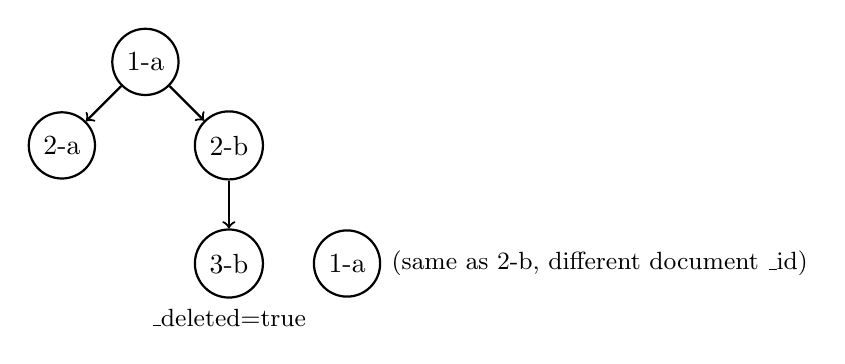
\begin{tikzpicture}[node distance={15mm}, thick, main/.style = {draw, circle}] 
      \node[main] (1) {1-a};
      \node[main] (2) [below left of=1] {2-a};
      \node[main] (3) [below right of=1] {2-b};
      \node[main, label=below:{\small \_deleted=true}] (4) [below of=3] {3-b};
      \node[main, label=right:{\small (same as 2-b, different document \_id)}] (5) [right of=4] {1-a};
      \draw[->] (1) -- (2);
      \draw[->] (1) -- (3);
      \draw[->] (3) -- (4);
  \end{tikzpicture} 
  \caption[Resolving a conflict by keeping both revisions]{Resolving a conflict by keeping both revisions --- \say{2-a} conflicts with \say{2-b} initially, then \say{2-b} is deleted, and a new document with a unique \_id is inserted (on the right), same as the deleted revision \say{2-b}}
  \label{graph:keep-both-resolution}
  \end{figure}

As it was mentioned earlier, all CouchDB documents have an $\_id$ and a $\_rev$ (as in \textit{revision}). When \textit{putting} a document --- CouchDB has a \textit{put} operation that allows insertions, edits and deletions, depending on the given argument --- if there is already an object with the same $\_id$, CouchDB will try to update it, however if the $\_rev$ does not match, a conflict is generated. For insertions, it only requires an object with at least an $\_id$ field. For edits, it requires the object with an $\_id$, referring to the document to be edited, and a $\_rev$, corresponding to the current revision of the document to be edited. For deletions, it requires the $\_id$, $\_rev$ and a $\_deleted$ field with a value of $true$, which is a special case of the edit operation. The deleted documents are not really removed from the database until a compaction operation\footnote{https://docs.couchdb.org/en/stable/maintenance/compaction.html} is performed to clean the deleted documents and older revisions are stripped, leaving only the necessary data required for conflict resolution operations.

Document revisions have two components: a number indicating their level in the tree of updates of that document, and a unique identifier. When a document is inserted, the generated revision starts with 1, and every time it updates, the successive revisions will have consecutive values e.g., 2, 3, and so on. This means that, considering two users are synchronized with the remote database which has a document with a revision of \say{1-xyz}, if they both want to update that document at the same time, they will both try to \textit{put} a document with \say{1-xyz} as its parent node. When CouchDB receives the requests, it will generate a revision for each, starting with 2, since their parent node revision starts with 1. One of them will be chosen as winner, and the other will conflict, since there are two documents on the same level: 2. The winner is automatically and deterministically chosen by CouchDB, so that every replica of the database is consistent, and it will store the conflicts for each document as well, then it's up to the application layer to resolve the conflict as needed. Figure~\ref{graph:couchdb-document-history} shows the history of a document's revisions, it starts on the revision level 1, then an edit generates the level 2 revision, and on the third level, there is a generated conflict, since two users tried to update it, by specifying the same root revision: \say{2-a}. CouchDB automatically chose revision \say{3-b} as the winner, but it still kept the \say{3-a} revision in memory. Figure~\ref{graph:couchdb-document-history-resolution} shows the same scenario, but adds the conflict resolution process, which works by deleting the revision we want to discard --- \say{3-b} in this case --- and since revision \say{3-a} becomes the only non-deleted leaf revision, it automatically becomes the winner and will be returned when someone fetches this document latest revision. The primary focus of this work starts here, by applying automatic conflict resolution strategies between the automatic CouchDB winner selection and the manual user conflict resolution that may happen afterwards.

\begin{figure}[h]
    \centering
    \begin{subfigure}[t]{.5\textwidth}
        \centering
        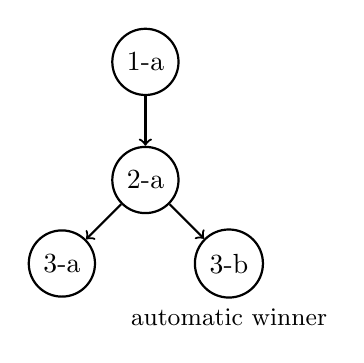
\begin{tikzpicture}[node distance={15mm}, thick, main/.style = {draw, circle}] 
            \node[main] (1) {1-a};
            \node[main] (2) [below of=1] {2-a};
            \node[main] (3) [below left of=2] {3-a};
            \node[main, label=below:{\small automatic winner}] (4) [below right of=2] {3-b};
            \draw[->] (1) -- (2);
            \draw[->] (2) -- (3);
            \draw[->] (2) -- (4);
        \end{tikzpicture} 
        \caption{Document revision history (conflict)}
        \label{graph:couchdb-document-history}
    \end{subfigure}%
    \begin{subfigure}[t]{.5\textwidth}
      \centering
      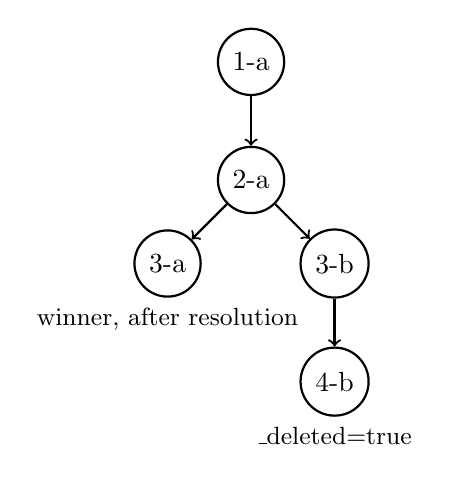
\begin{tikzpicture}[node distance={15mm}, thick, main/.style = {draw, circle}] 
        \node[main] (1) {1-a};
        \node[main] (2) [below of=1] {2-a};
        \node[main, label=below:{\small winner, after resolution}] (3) [below left of=2] {3-a};
        \node[main] (4) [below right of=2] {3-b};
        \node[main, label=below:{\small \_deleted=true}] (5) [below of=4] {4-b};
        \draw[->] (1) -- (2);
        \draw[->] (2) -- (3);
        \draw[->] (2) -- (4);
        \draw[->] (4) -- (5);
    \end{tikzpicture} 
    \caption{Document revision history (conflict) with conflict resolution}
    \label{graph:couchdb-document-history-resolution}
    \end{subfigure}
    \caption{Document revision history --- CouchDB model}
    \end{figure}

\subsection{Base conflict resolution strategies}

A base set of operations was defined in order to help solve conflicts. As per design, every conflict is resolved individually, i.e., if there are three documents conflicting, the conflict resolution will take place two times, one for each conflict pair (current winner, conflict). They all receive the pre-selected winner and conflict documents as arguments:
\begin{description}
    \item[\textbf{Leave Conflict}] This is the most basic resolution operation. It does nothing and leaves the conflict in the database, so that it can be resolved later in the frontend application;
    \item[\textbf{Ignore Conflict}] This is another basic resolution operation. It simply deletes the conflicting revision, basically agreeing with the automatic decision done by CouchDB;
    \item[\textbf{Choose a Winner}] This operation deletes the document passed as conflict and inserts a new revision as the winner;
    \item[\textbf{Keep Both}] This operation resolves conflicts by keeping both documents. Since there can't be two documents with the same id in CouchDB, otherwise they would conflict, it first deletes the conflicting revision, creates a new revision for the current winner, and inserts a new document equal to the conflicting one, but with a UUID\footnote{A UUID (Universally Unique Identifier) is a random 128-bit identifier. \cite{uuid-rfc}} appended to its default id. This ensures that it won't conflict with the existing document, however it has the downside that it won't conflict with anything ever again. While the initial document remains in the database, there will always be a \say{representative} of that set of ids, that will trigger conflicts every time a new document with that id is inserted. If that document is deleted, there is a workaround in place that selects a document from those with the same base id, and removes the random suffix, so that there is always some event to detect the conflicts for future inserts;
\end{description}

Additionally, there are specific resolutions that are triggered on the frontend --- not automatically ---- if the user resolves a conflict by choosing a winner or by keeping all conflicting documents:

\begin{description} \label{list:conflict-resolution-strategies-frontend}
    \item[\textbf{Choose One --- Frontend}] When choosing a winner, since there may be multiple conflicts at the same time, it needs to delete them all to fully resolve the conflict. However, if multiple users select different winners by each resolving the conflict differently, in the end they would end up deleting all documents. In order to avoid this, after deleting the loser documents, a new revision for the winner is inserted, so that if those multiple users select different winners locally, their choices will still conflict with each other after each \say{round} of conflict resolution. 
    \item[\textbf{Keep All}] This operation is similar to the \textit{Keep Both} operation in concept, but applied to $n$ documents at a time, not only 2 documents. It does so by first deleting all conflicts corresponding to a document id, then inserting new documents equal to the deleted conflicts, but with a UUID appended to the id, to make them unique, and avoid the conflict;
\end{description}

\subsubsection{Composite conflict resolution strategies}

By leveraging the aforementioned strategies, it's possible to create complex rules that apply to different event types that conflict with each other, provided that they happen in the same match minute and belong in the same event category.

\begin{description}
    \item[\textbf{Force Winner By Event Id}] Chooses as winner the document that has a given event id;
    \item[\textbf{Highly Conflicting; Ignore if same player}] If the player is the same, ignore conflict; Otherwise leaves the conflict intact to be resolved by the user;
    \item[\textbf{Goal vs. Own Goal}] In case a user reports a goal from team A, but another reports own goal from team B, they are both referring to the same goal, so the own goal event is chosen as winner, since it is more specific. Otherwise, leave the conflict to be resolved by the user;
    \item[\textbf{If same player, keep the one with given event id}] If the events refer to the same player, choose as winner the one that has the given event id; Otherwise leave the conflict to be resolved by the user;
    \item[\textbf{If different player, use reputation; Otherwise ignore}] If the referred players are different, choose as winner the event whose user has the highest reputation; Otherwise, ignore conflict;
    \item[\textbf{If same player, use reputation; Otherwise, keep both}] If the referred players are the same, choose as winner the event whose user has the highest reputation; Otherwise, keep both documents;
    \item[\textbf{If same player, ignore conflict; Otherwise, keep both}] If the referred players are the same, ignore the conflict; Otherwise, keep both documents;
    \item[\textbf{If same player, ignore conflict; Otherwise use reputation}] If the referred players are the same, ignore the conflict; Otherwise, choose as winner the event whose user has the highest reputation;
    \item[\textbf{Substitution Handler}] If the involved players are the same, ignore the conflict; If there are intersecting players, i.e., an event mentions player A out for player B, and the other event mentions player A out for player C, the conflict is left intact to be resolved by the user, later. Finally, if the involved players are different, keep both documents;
    \item[\textbf{Minute based resolution}] Receives a $minuteCondition$ function that takes the documents' minute as argument, a resolution function to execute if true, and a resolution function to execute if false. If $minuteCondition$ returns true, the first function is called, otherwise the second one is called;
    \item[\textbf{Choose biggest reputation}] Choose as winner the event whose user has the highest reputation;
\end{description}

\subsubsection{Synchronization with ZeroZero API} \label{sec:api-sync}

In order to fulfill User Stories \ref{user-story:sync-to-api} and \ref{user-story:sync-from-api}, specific logic was implemented to fetch missing events from the API, and to add them after consensus is reached on the ZeroZero Live platform i.e., there are no conflicts.

That being said, on the same loop that listens for changes and verifies if there are conflicts to resolve, the handler also two more branches of action: when the event is being synced from the API into CouchDB, and when the event has no conflicts and was not synced from the API.

Starting with the latter, the handler needs to know which operation was done regarding each event, in order to call the correct ZeroZero API. Each document comes as if we were receiving a CouchDB's \say{put} call, meaning that we don't know explicitly if it was an insert, edit or delete. In order to know if it is a delete operation, we can check for the $\_delete$ field. As was mentioned earlier, this field is true when the document is deleted. Regarding the distinction between inserts and edits, it's not as simple. On a first approach, revisions were used: if the revision level was 1, it was obviously an insert, otherwise it would be an edit to some existing document. This seemed rational, and it works to some extent, but not always. Recalling CouchDB delete behavior explained above, documents are not really deleted until the compaction operation is run. That means that if a document is deleted, another with the same id can be inserted afterwards, but since the first was not really erased from the database, the revision level of the newly inserted event will actually be different than 1, since the history for that document id is still there. In this case, this approach would consider some inserts as edits which would cause multiple events from being synchronized to the API correctly. In order to fix this, a special flag was added to each document, meaning if the document was meant to be inserted or not. On the client side, every event creation would generate a document with the $insert$ flag with a value of $true$. Whenever the handler inserted a document, it would edit it --- create a new revision --- setting the $insert$ flag back to $false$, so that it was not inserted every time there were changes to it. The final approach was then to check for the $insert$ flag in order to distinguish from insert and edit operations.

Regarding the synchronization from the ZeroZero API --- their internal storage of events, managed by the older platform, and used to show the match events on their website --- into ZeroZero Live, it's a bit more complex. First it shouldn't be continuous, or it would easily cause problems, since we would be adding events there and immediately receiving them back would probably cause some unwanted conflicts. With this in mind, every time there is a match page load --- on first visit, or on page refresh --- for every event that is on the ZeroZero API that has no correspondent document on CouchDB, there will be a synchronization attempt in order to add it to the CouchDB database. The reason because this is not as simple as inserting every event that is currently not in the ZeroZero live database yet, is because of potential conflicts: Events that are already on the ZeroZero side, should not conflict with each other, and they also should not conflict with CouchDB documents, on the synchronization phase, at least.

First, let's explain how events are known to be synchronized or not. Every time there is an insert of a document on ZeroZero Live, and it is synchronized \textit{to} the ZeroZero API --- as per the logic described above --- the API returns an id for that event, that is different from the document's $\_id$. That id is used identify the event on the ZeroZero side, allowing us to call the edit and delete APIs on the events. When the CouchDB document is synchronized to the ZeroZero API --- the insert API is called ---, the document is edited to set the $insert$ flag to false, as mentioned above, but it also sets the $id$ field, meaning that the document has a ZeroZero's event counterpart.

Based on this, for every event coming from the ZeroZero API, we can check if there is a CouchDB document with a corresponding $id$, if there isn't, that event needs to be inserted into CouchDB.

For those that need to be synchronized, they are inserted as normal documents, as if they were inserted by the user, however, the document $\_id$ has an appended \say{synced\_from\_api} suffix, so that the handler will know to use the synchronization algorithm, instead of simply inserting the event.

\begin{figure}[h]
    \begin{center}
        \leavevmode
        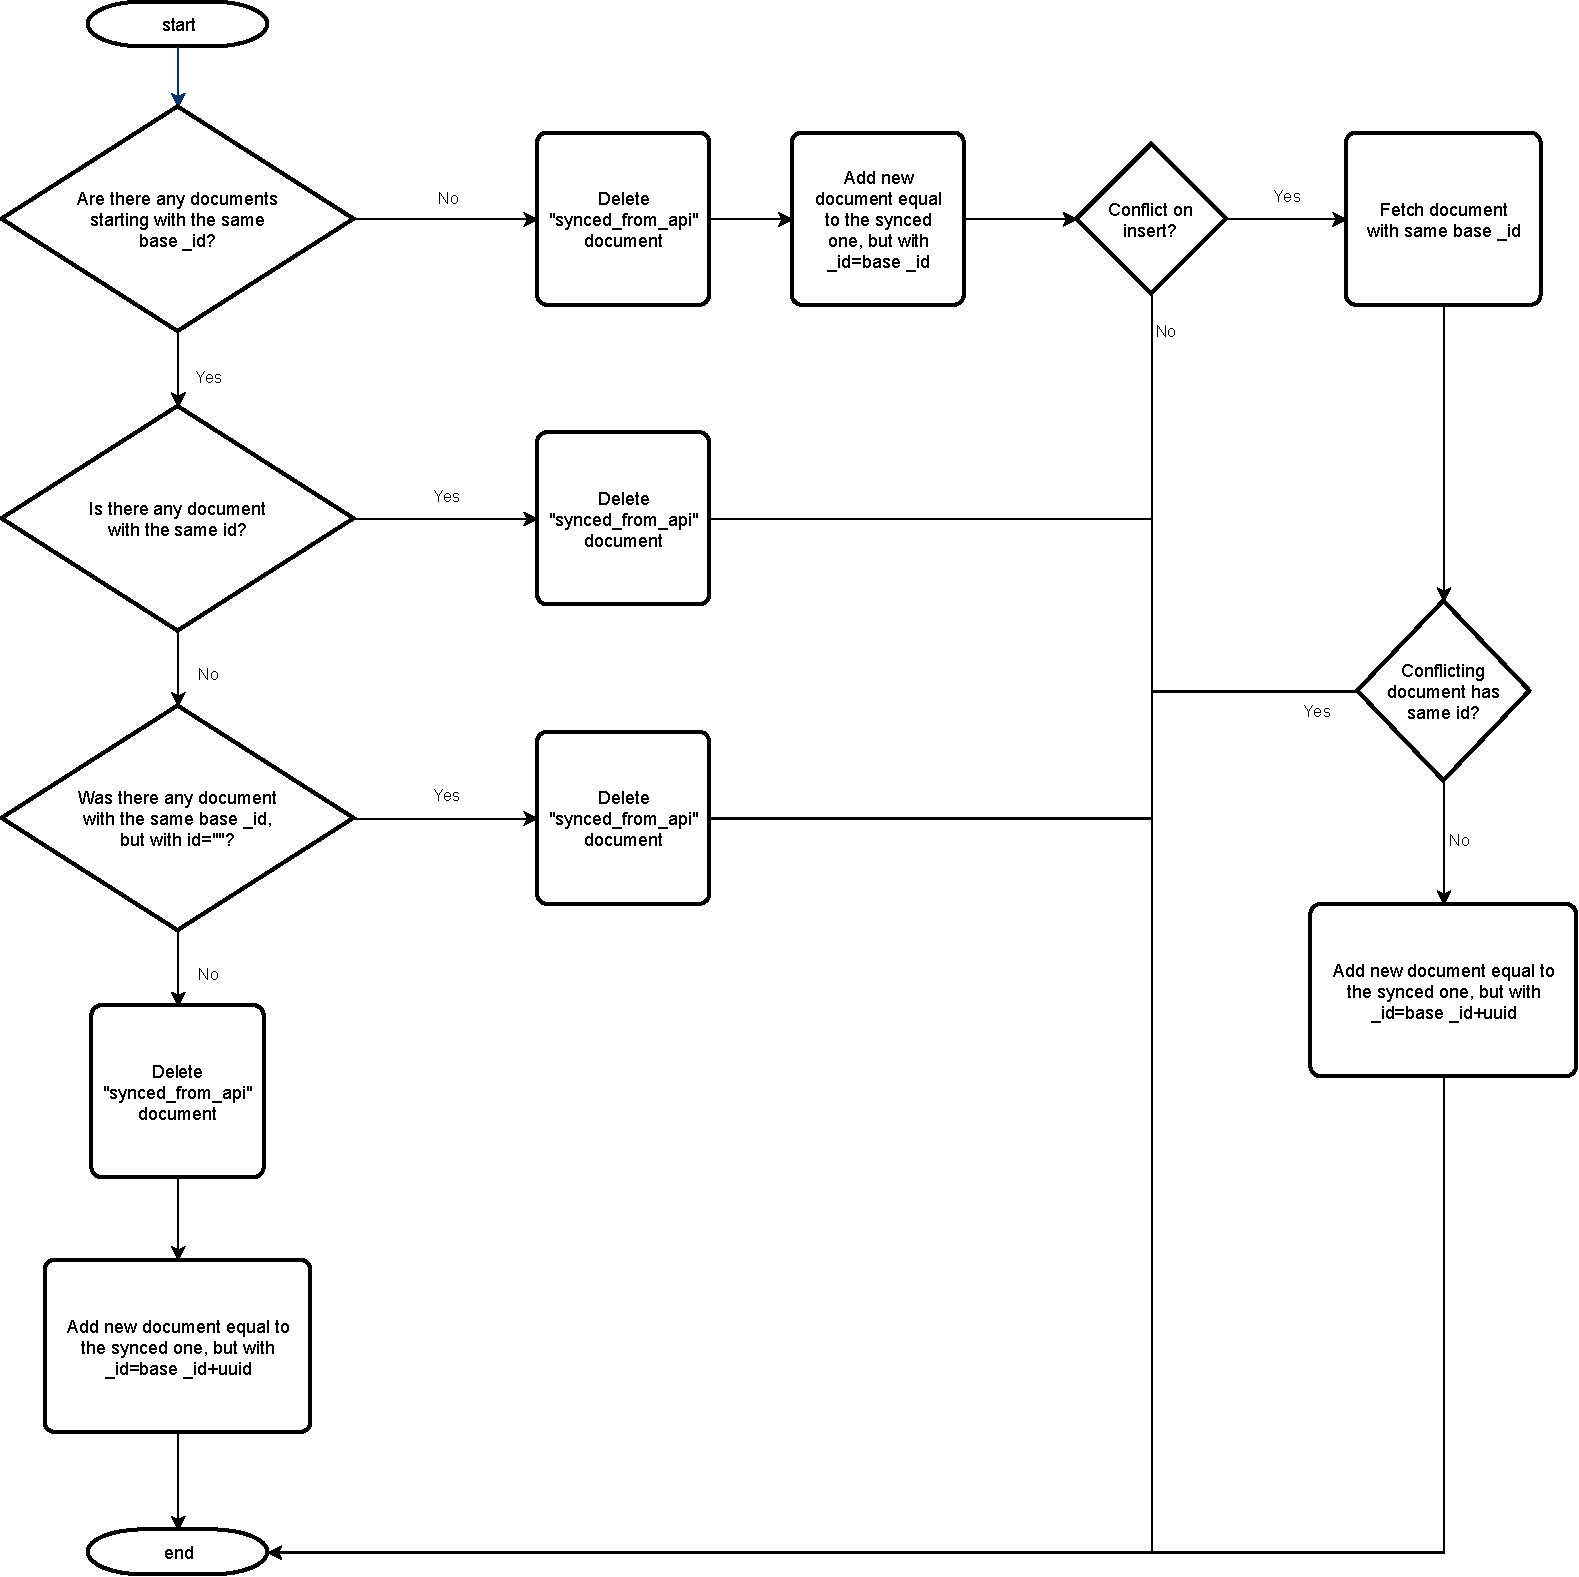
\includegraphics[width=\textwidth]{sync-api-flow.pdf}
        \caption{Synchronization of events from ZeroZero API into ZeroZero Live database}
        \label{fig:sync-from-api-flux}
    \end{center}
\end{figure}

Figure \ref{fig:sync-from-api-flux} shows the flowchart relative to the algorithm of synchronization of events into CouchDB. It first checks if there are documents starting with the same base $\_id$. The base $\_id$ is the $eventMinute-eventMinuteExtra-eventCategory$ string used to identify documents and allow for conflict detection. Due to custom resolutions like \textit{Keep Both} or specific document types that never conflict --- such as comments --- some documents will have a base $\_id$ followed by a unique part, in UUID format, thus it's important that it is ignored, otherwise some events would never be caught by the synchronization algorithm. It's also important to note that even if there is a document with a same base $\_id$, they may not refer to the same event, and not even correspond to the same event type, it just means they happened at the same minute, and belong to the same event category. The only way there is to know if a synchronization candidate --- i.e., the one with \say{synced\_from\_api} appended to the $\_id$ ---  is the same as an existing document, is by comparing their $id$s, not $\_id$s, as that value comes from the ZeroZero API.

First, if there are no documents in the CouchDB database that have a same base id, we can know for sure that that event is not in the CouchDB database yet, thus, the \say{synced} document is deleted, and a clone is inserted with the correct $\_id$ --- i.e., the base $\_id$ --- so that it can conflict in the future with other events. However, imagine that while this is happening, someone inserts an event at the same minute with the same category. That will prevent us from inserting the new version of the \say{synced} document, so there is a check in place that verifies the conflicting document and if it has the same id, the algorithm stops, since the event is already there, otherwise, it will add it, but with a unique UUID suffix, so as to avoid the conflict on insertion.

If there are any documents with the same base $\_id$, however, it will try to find out if among those there is some that has the same id. If so, it will simply delete the \say{synced} document, it is already synchronized. If not, and if among the searched documents there's some that have an empty id --- meaning they are in the middle of the process of getting one, after the insert call --- the algorithm will delete the \say{synced} document as a preemptive measure, hoping it will be there in the future. The next time this algorithm runs, that document will already have an id, and the check above can be done.

Finally, if there were documents with the same base $\_id$, but none had the same id nor had empty ids, the synchronization candidate is not present, but must be added with an unique suffix, to prevent insertion conflict.

\subsection{Conflict Handling Orchestrator}

In order to have multiple handlers at once, which is needed as there may be multiple matches happening at the same time, one needs to have a controller that handles their initialization, manages their status and stops them once they are not needed anymore.

That is the responsibility of the Conflict Handling Orchestrator. It is a simple Node.js application that exposes an HTTP API, that lets us initialize a conflict handler for a given match, list active handlers, stop a conflict handler for a given match, and \textit{kill} any \textit{zombie} handler references that might be left over after a crash. The state of the handlers is kept in a LevelDB\footnote{https://github.com/google/leveldb} database, which is a simple key-value database. Each record will have the match id as the key and the value is an object containing the PID of the handler process for that match, as well as the timestamp of when the handler was started.

Even though the orchestrator is the parent process of the conflict handlers, in case the conflict handler process fails, the orchestrator is independent enough that it won't terminate as well. If the orchestrator itself fails for some reason, it is built to auto-restart instead of making the docker container restart, which would make it lose context and terminate all other processes, including child conflict handlers. This is why information about the handlers is kept in a separate database, instead of in-process memory, so that the orchestrator can recover all of it in case of failure.

\paragraph{POST /initConflictHandler/:matchId}
This endpoint launches a child process running a conflict handler for the specified match, as described in the previous subsection. It is made in such a way that it won't allow the launch of multiple handlers for the same match simultaneously. After a specified timeout, the child process is killed, to avoid wasting resources on finished matches.

\paragraph{POST /stopConflictHandler/:matchId}
This endpoint terminates a process associated with the given match.

\paragraph{GET /active-handlers}
This endpoint returns a list of active match conflict handlers, together with their respective PIDs.

\paragraph{POST /cleanup-zombies}
This endpoint will verify that every stored match handler is actually running. If not, it will update the database. This is important because after some failure, conflict handlers might not be running as the database shows, and this endpoint will restore the truth.

\section{Reputation Service}

In order to aid the automatic conflict resolution, in many cases, the reputation of the users will be used to determine which event to choose as the conflict winner. This is only done for conflicts that are not critical. For any important conflict --- such as \textit{Goal from team A} vs. \textit{Goal from team B} --- it is left for users to resolve manually on the UI.

The Reputation System is based on the fact that people that input conflicting events disagree with each other, as well as who edits or deletes an event. Every time a user receives an event from someone, they implicitly agree with it, until they act to mark disagreement, executing any of the actions described before. Finally, users can explicitly agree with each other, by inputting conflicting events, that are exactly the same i.e., if two users report a goal from team A at the same time, they are not disagreeing with each other, but rather agreeing. This is considered a more \textit{powerful} agreement, since they both explicitly inputted the event, instead of just waiting for someone to do it and passively reading it. These are the three interaction types that are registered by the reputation service.

The Reputation Service is a Node.js microservice that exposes an HTTP API, and uses a \mbox{MongoDB} database to persistently store data. It has endpoints to register interactions between users and inputs and another endpoint to calculate reputation updates after a specific match interactions. MongoDB was chosen due to its good horizontal scaling ability, which is useful for future-proofing the application, without losing too much performance currently. Additionally, there's a lack of relationships between the collections, thus an SQL-based alternative is not necessary.

The database will store the interactions, which are documents containing the $matchId$, $eventId$, $userId$, $eventOwnerId$, $isProcessed$ and $interactionType$ fields. $matchId$, $eventId$, and $userId$ uniquely identify an interaction and are used to prevent the same user from registering multiple interactions for the same event. Additionally, there are checks in place so that a user cannot register interactions for an event they have inserted. $isProcessed$ is a boolean flag that marks the interaction as processed by the reputation calculation, so that it is not used multiple times when calculating reputation updates. Finally, the $interactionType$ defines the type of interaction, which affects the reputation update calculation, e.g., $Agree$, $Disagree$, $Explicit Agree$

Additionally, the database has another collection to store the user and their respective reputations, to be used in the conflict resolution. Each document has $userId$, $reputation$ and $updatedAt$ fields. The $reputation$ represents the numerical value of the reputation of the user with id $userId$, and the $updatedAt$ field is used to calculate the reputation decay --- the more time passes after the previous reputation calculation, the more its reputation will decay due to inactivity.

\paragraph{GET /:userId/reputation}

This endpoint returns the current reputation for the given user.

\paragraph{POST /:matchId/:eventId/:eventOwnerId/:userId/agree}

This endpoint is called every time a user receives an event in their local database. It means that they \textit{implicitly} agree with that input, since they haven't yet done something else to manifest any intention on the contrary. Like the other interactions, it does not allow self-voting, and is overwritable, meaning of course that once a user wants to disagree with some input, the previous implicit agreement will be nullified. Finally, it cannot overwrite any existing interaction on the same input, since this endpoint is made to be called automatically, it can be done without worrying about overwriting any other explicit interactions.

\paragraph{POST /:matchId/:eventId/:eventOwnerId/:userId/disagree}

This endpoint is called every time a user edits or deletes an event, or when there is a conflict. It means that the user \textit{implicitly} explicitly disagrees with that input, since they have done something to manifest any intention. Like the other interactions, it does not allow self-voting, but it is not overwritable, meaning that once a user disagrees with some input, that disagreement is forever. Finally, it can overwrite any existing interaction on the same input, since this endpoint is made to be called explicitly, after any automatic interactions may have been recorded.

\paragraph{POST /:matchId/:eventId/:eventOwnerId/:userId/explicit-agree}

This endpoint is called every time a user inserts and event that conflicts with another event that is essentially the same. It means that, even though the events conflict, they are the same, so both users are explicitly agreeing with each other. Like the other interactions, it does not allow self-voting, but it is not overwritable, meaning that once a user explicitly agrees with some input, that agreement is forever. Finally, it can overwrite any existing interaction on the same input, since this endpoint is made to be called explicitly, after any automatic interactions may have been recorded.

\paragraph{POST /:matchId/updateRep}

This endpoint calculates and updates the reputation of the users involved in a specific match. It runs the reputation algorithm that uses the stored interactions to calculate a new reputation for each user. The algorithm is based on the ideas presented in Section~\ref{sec:rep-sys-sota}, as it takes into account the different types of interactions as well as a reputation decay over time.

First, for every user involved in the match, it will calculate a reputation decay multiplier based on the last time the reputation was calculated for that user --- users that stay inactive for longer get a bigger penalty. 

\begin{equation}
    newUserRep = oldUserRep * decayCoefficient^{timeSinceLastUpdate}
\end{equation}

Then, for every recorded interaction, it will calculate the set of deltas that corresponds to the effect of a specific interaction on a specific input. Different interactions result in different deltas.

For agreements:
\begin{equation}
    deltaA = baseInputRep * maxRepReward * userRep * userRepInfluence
\end{equation}

For disagreements:
\begin{equation}
    deltaD = -baseInputRep * (1 - (maxRepReward * userRep * userRepInfluence))
\end{equation}

For explicit agreements:
\begin{equation}
    deltaEA = (deltaAgreement) * (1 + explicitAgreementBonus)
\end{equation}

After calculating all the deltas for each interaction, they are marked as processed, to avoid being used mutiple times when calculating reputation updates. Users' reputations are then updated according to the average of the deltas of their concerning interactions:

\begin{equation}
    repIncrement = (1 - userRep) * avgDeltas;
\end{equation}

\begin{table}[h]
    \centering
    \caption{Reputation service constant values}
    \begin{tabular}{|l|l|l|l|}
        \hline
        \textbf{Constant}                   & \textbf{Value} \\ \hline
        Initial User Reputation             & 0.2 \\ \hline
        Base Input Reputation               & 0.01    \\ \hline
        Maximum Input Reputation Reward     & 0.05    \\ \hline
        Maximum Input Reputation Punishment & 0.1    \\ \hline
        User Reputation Influence           & 0.2    \\ \hline
        Explicit Agreement Bonus            & 0.2    \\ \hline
        Reputation Decay Coefficient        & 0.85    \\ \hline
    \end{tabular}
    \label{table:reputation-constants}
\end{table}

The used constant values are defined in Table~\ref{table:reputation-constants}. With this configuration, it takes approximately one month --- 4 weeks --- for a user to lose half of their reputation.

\section{Web Application (Frontend)}

The last component, and arguably the most important --- How would users use the application otherwise? --- is the frontend web application. For browsers, it's a set of HTML, CSS and JavaScript files being served by an Nginx web server. Many web applications have this setup, but let us dive deeper on the process that happens before the generation of those files to be served.

The application is built with React and is essentially a \textit{Single Page Application} (SPA), but regardless of the nomenclature, the application provides multiple interfaces, or pages. It doesn't work like the usual multi-page web application, since there is indeed only one page being served --- index.html --- however, the JavaScript, namely the React Router package, handles the routing and the URLs, by rendering different component trees based on the URL, and thus emulating a multi-page setup.

\begin{figure}[h]
    \begin{center}
        \leavevmode
        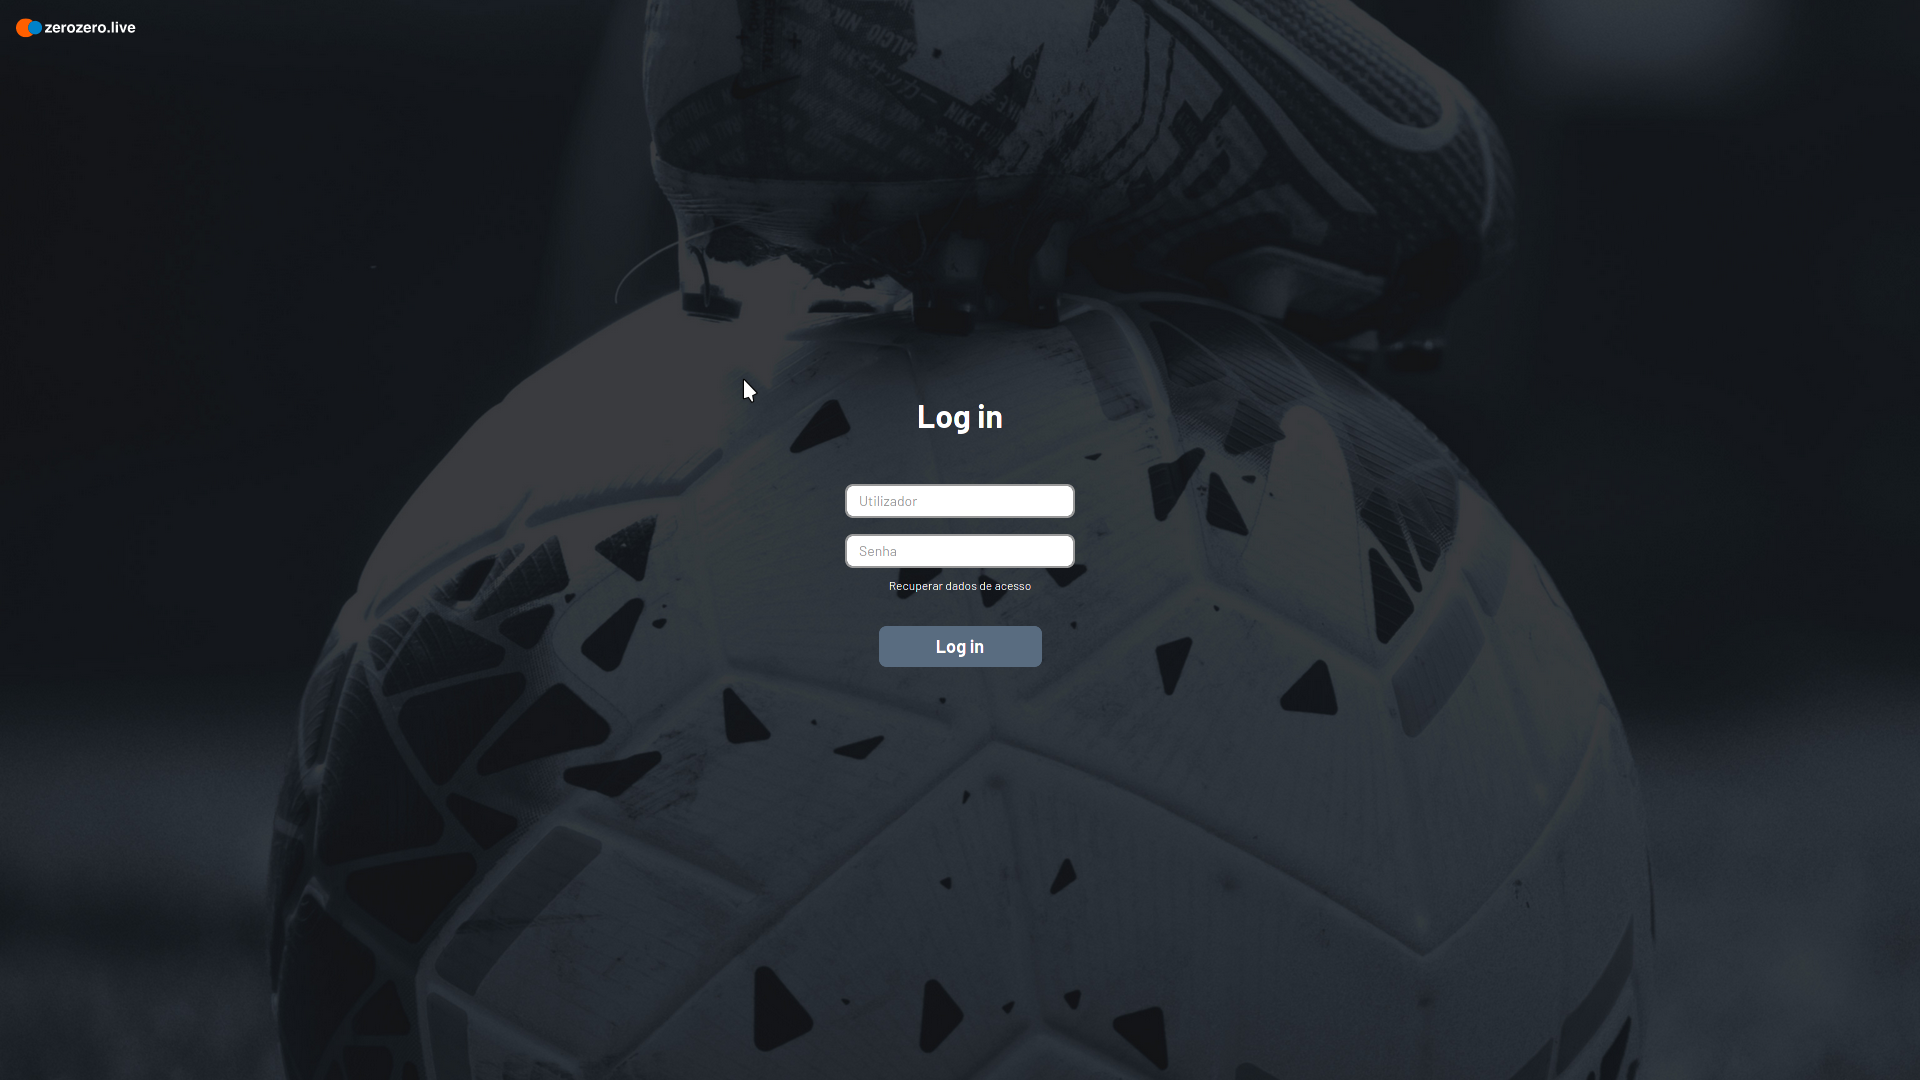
\includegraphics[width=\textwidth]{zerozerolive-login.png}
        \caption{Login page of zerozero.live}
        \label{fig:zerozerolive-login}
    \end{center}
\end{figure}

\begin{figure}[h]
    \begin{center}
        \leavevmode
        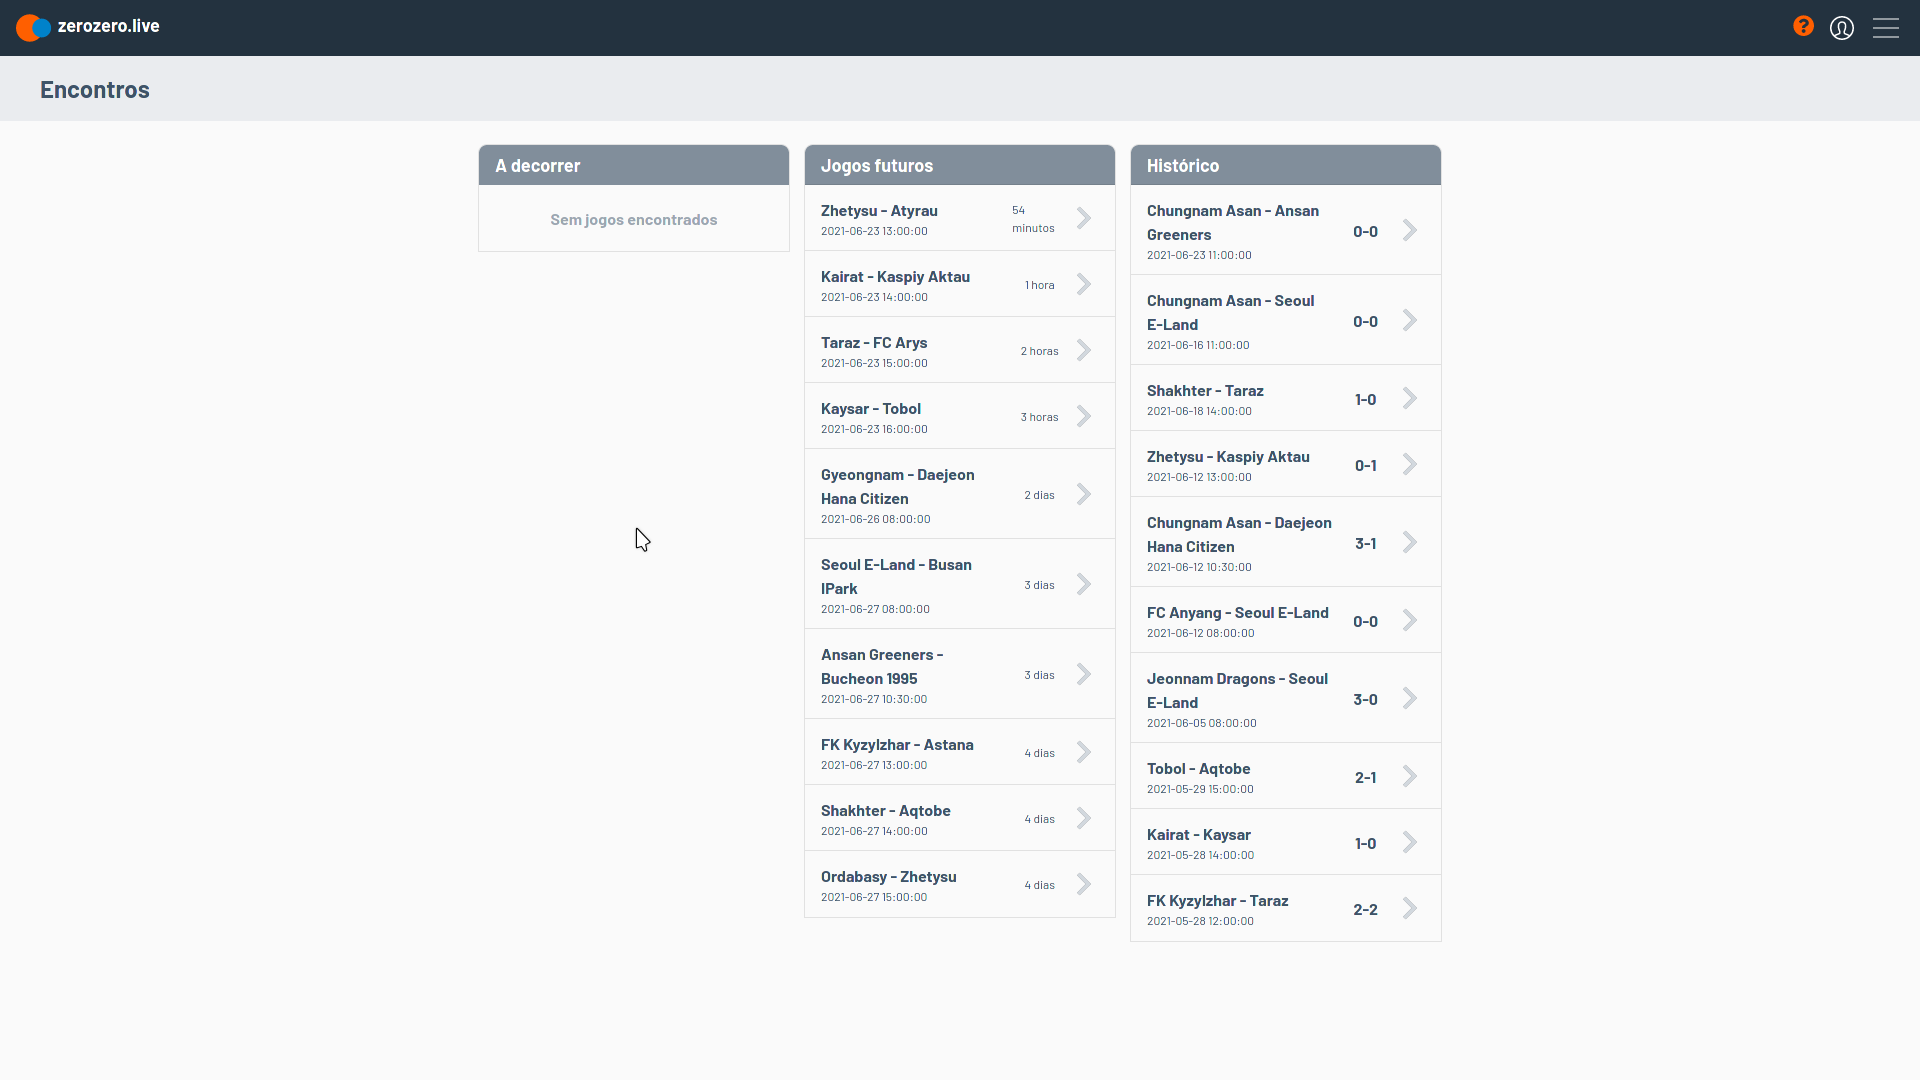
\includegraphics[width=\textwidth]{zerozerolive-home.png}
        \caption{Homepage of zerozero.live}
        \label{fig:zerozerolive-home}
    \end{center}
\end{figure}

\begin{figure}[h]
    \begin{center}
        \leavevmode
        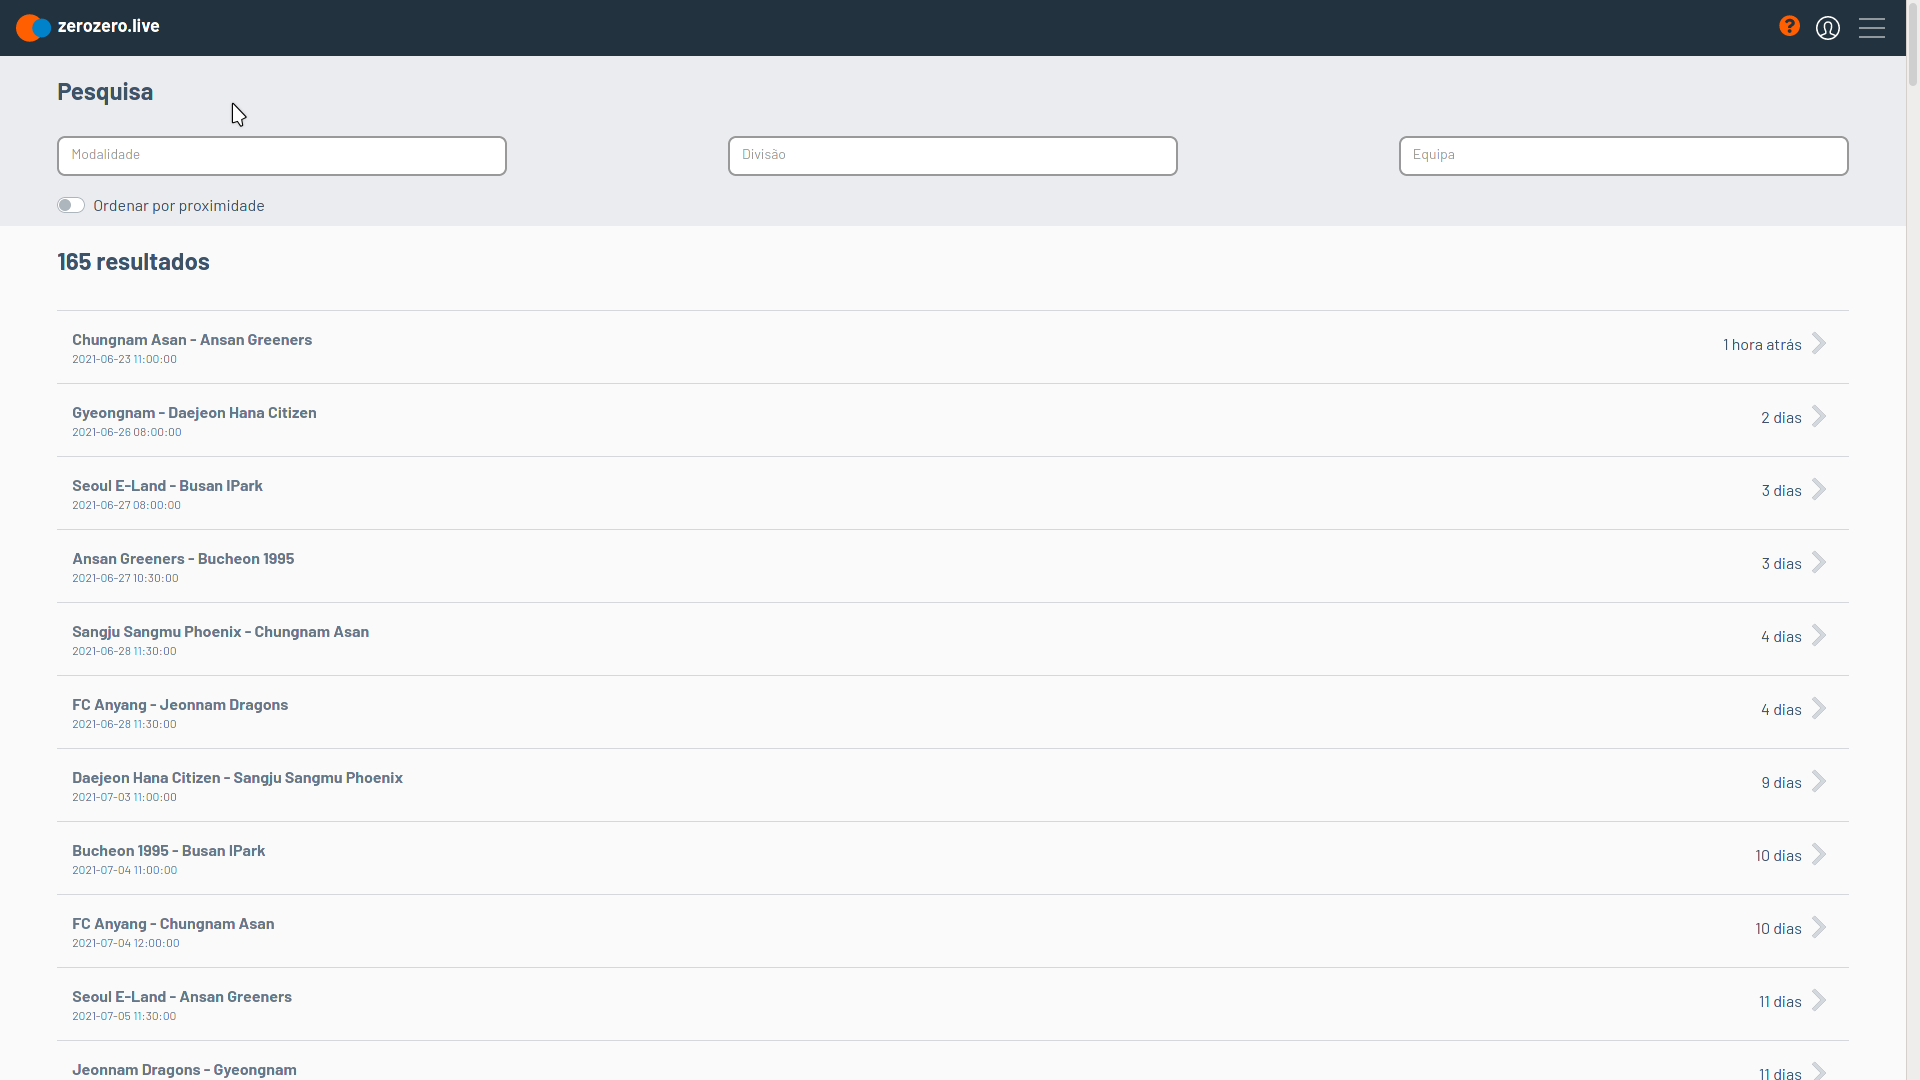
\includegraphics[width=\textwidth]{zerozerolive-search.png}
        \caption{Search page of zerozero.live}
        \label{fig:zerozerolive-search}
    \end{center}
\end{figure}

\begin{figure}[h]
    \begin{center}
        \leavevmode
        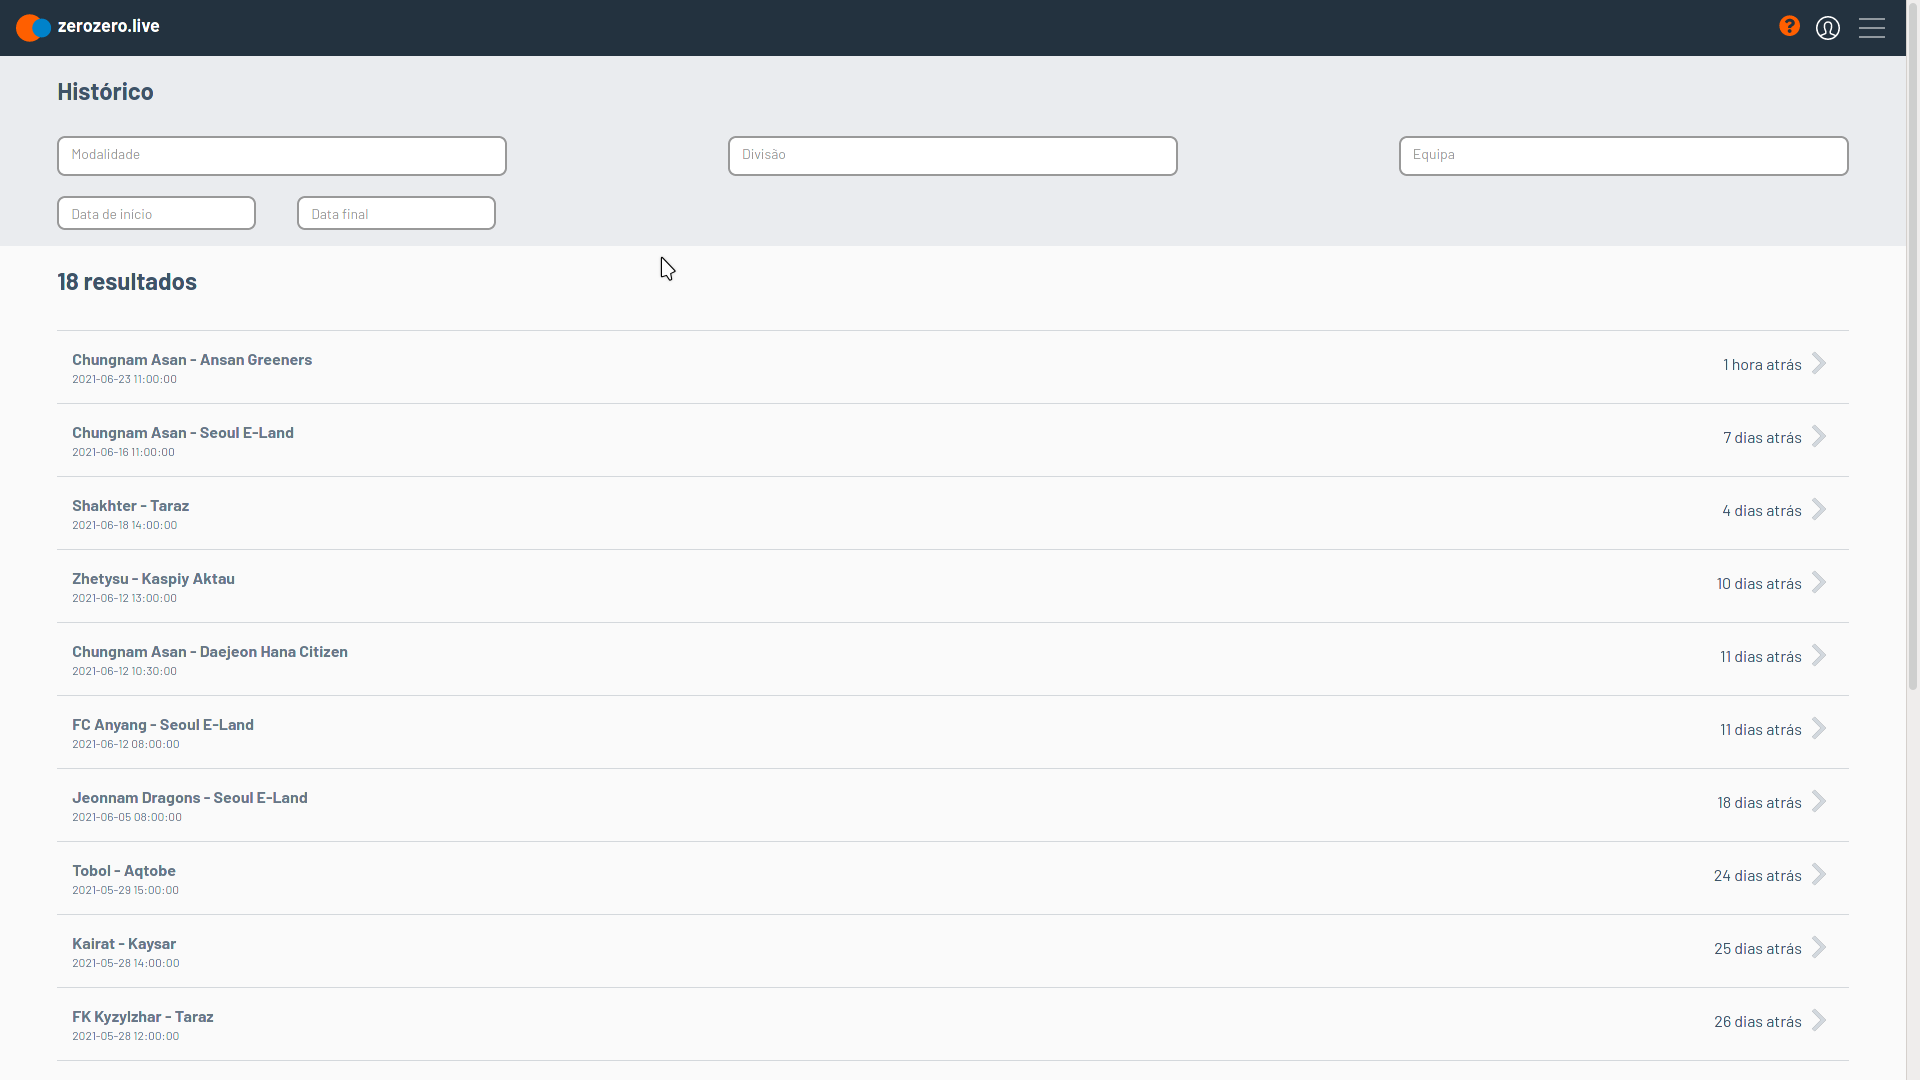
\includegraphics[width=\textwidth]{zerozerolive-history.png}
        \caption{History page of zerozero.live}
        \label{fig:zerozerolive-history}
    \end{center}
\end{figure}

\begin{figure}[h]
    \begin{center}
        \leavevmode
        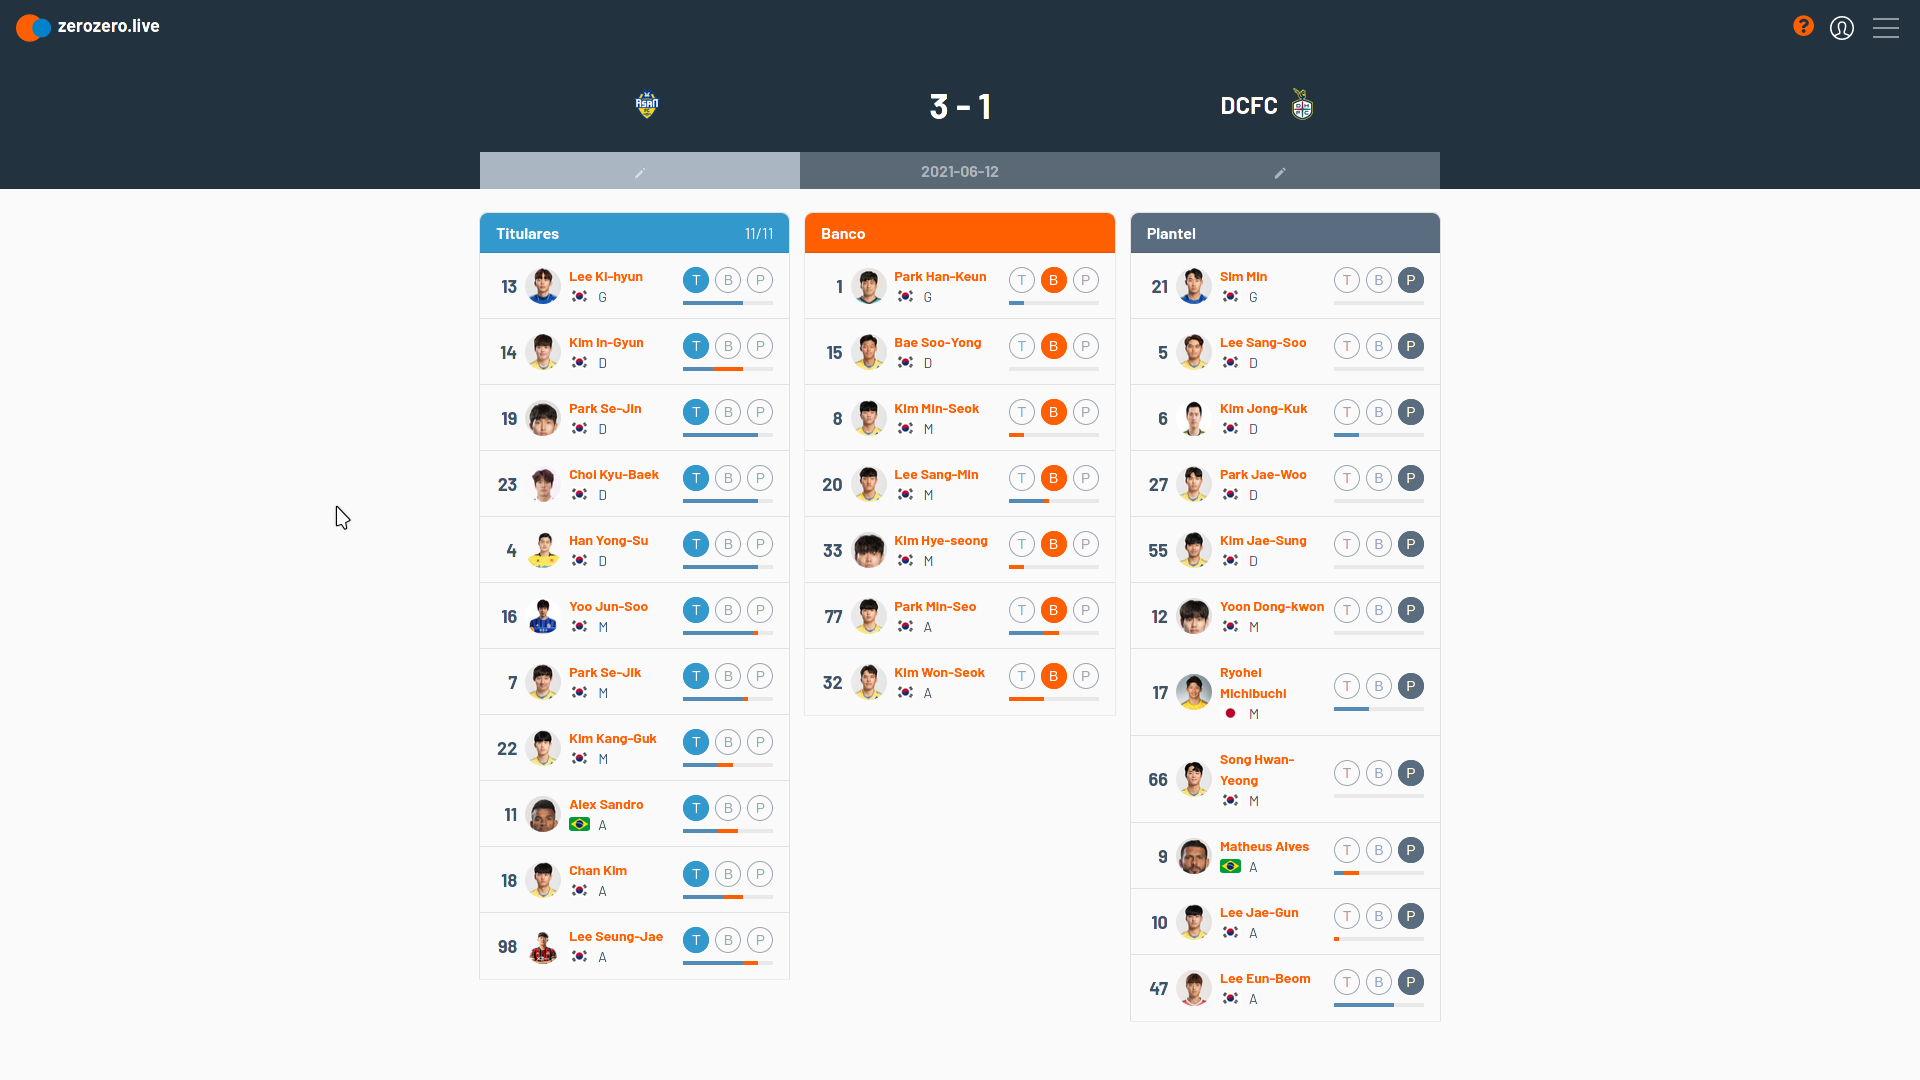
\includegraphics[width=\textwidth]{zerozerolive-teams.png}
        \caption{Team selection for a match in zerozero.live}
        \label{fig:zerozerolive-teams}
    \end{center}
\end{figure}

The majority of the frontend application was already built before. Figures~\ref{fig:zerozerolive-login}, \ref{fig:zerozerolive-home}, \ref{fig:zerozerolive-search}, \ref{fig:zerozerolive-history} were mostly untouched during the development of this work, as they are of no interest to the real-time multi-user collaboration problem this work addresses. Figure~\ref{fig:zerozerolive-teams} shows the interface to pick the roster of each team. There were no major changes to it apart from fixing an issue where users could not change pages too fast, as it might not submit their information correctly.

\begin{figure}[h]
    \begin{center}
        \leavevmode
        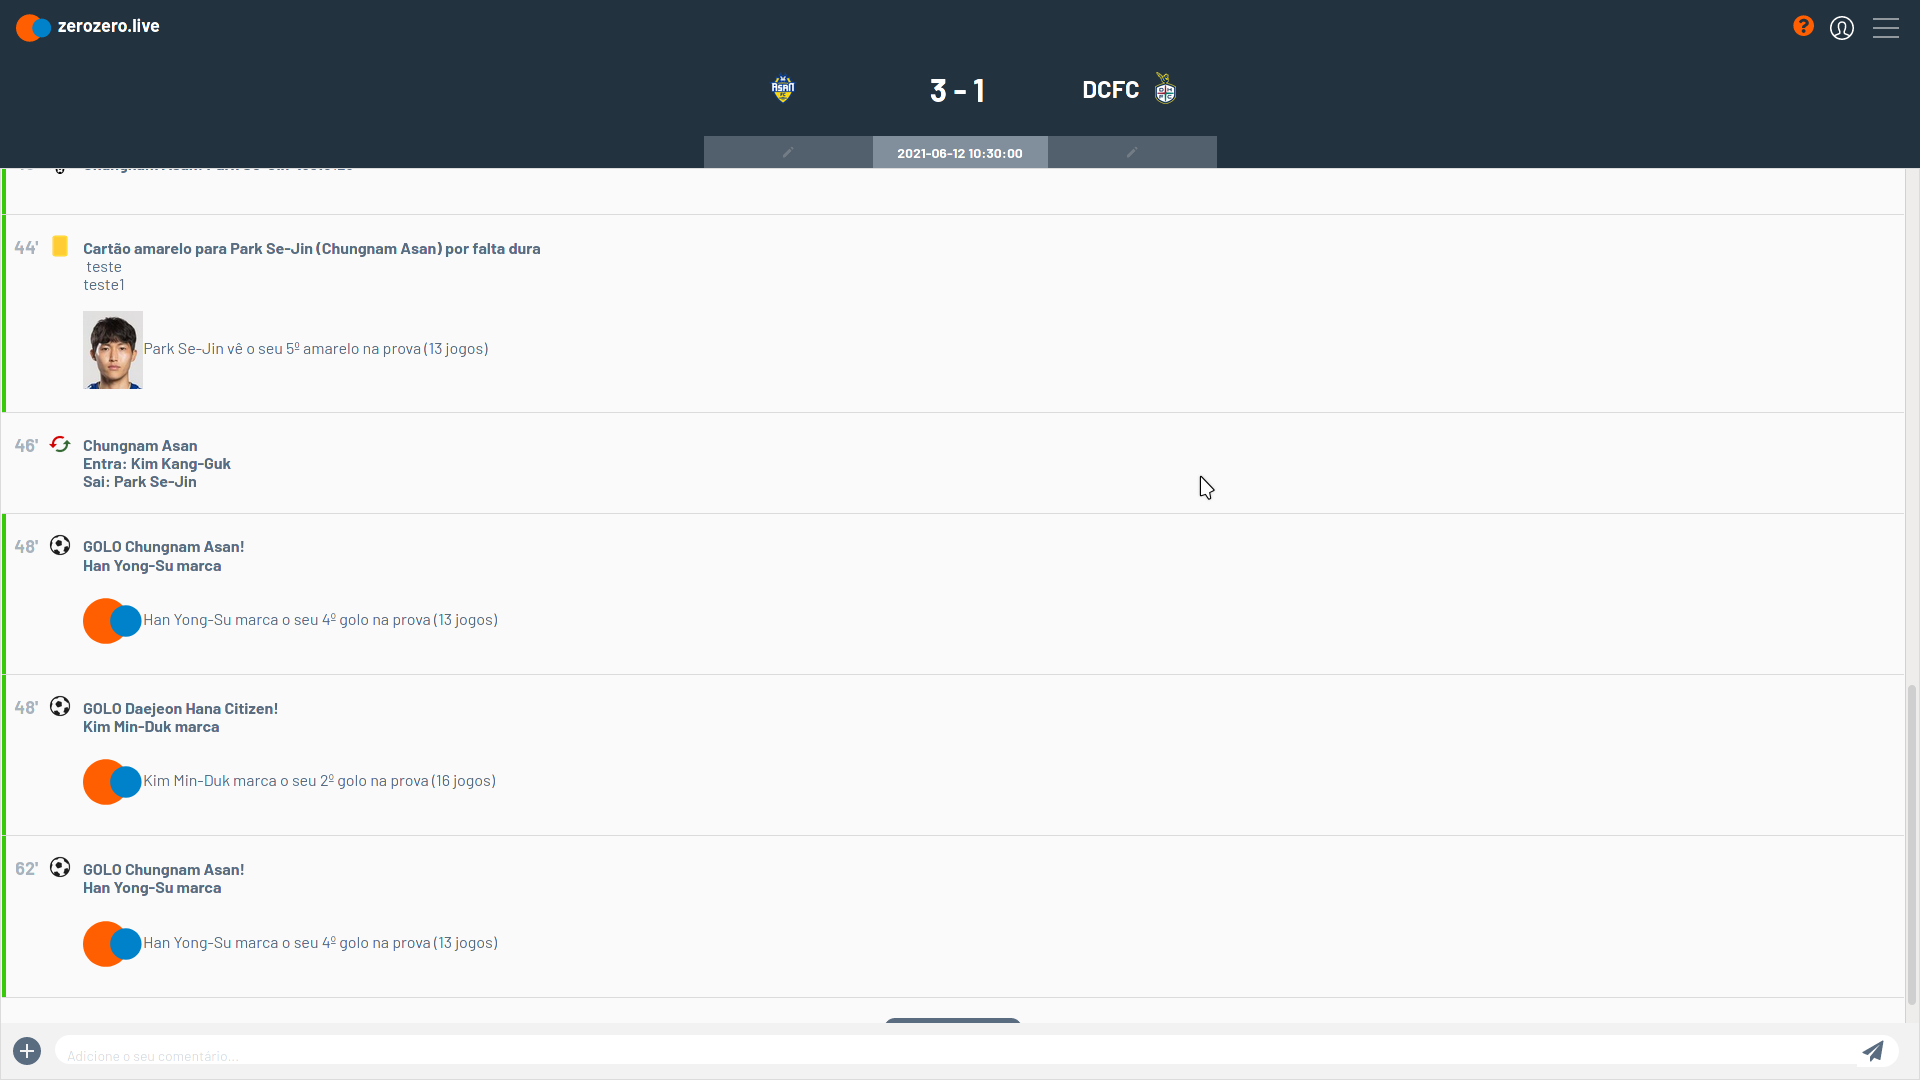
\includegraphics[width=\textwidth]{zerozerolive-comments.png}
        \caption{Comments page for a match in zerozero.live}
        \label{fig:zerozerolive-comments}
    \end{center}
\end{figure}

\begin{figure}[h]
    \begin{center}
        \leavevmode
        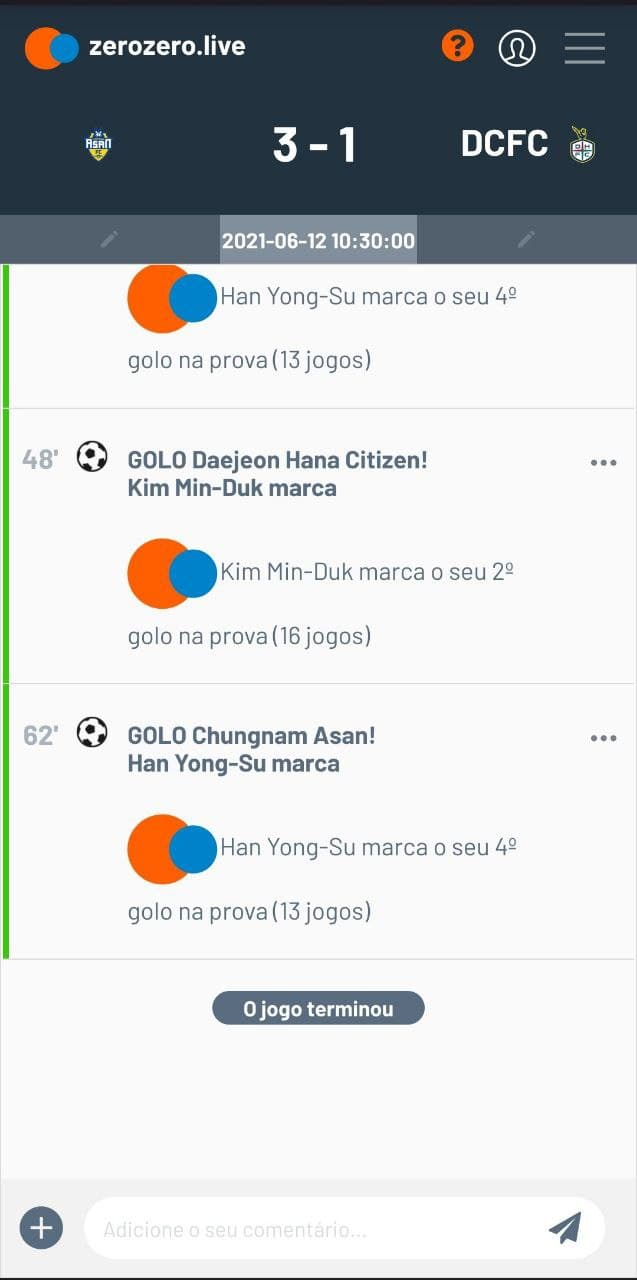
\includegraphics[width=0.3\textwidth]{zerozerolive-comments-mobile.jpg}
        \caption{Comments page for a match in zerozero.live --- Mobile version}
        \label{fig:zerozerolive-comments-mobile}
    \end{center}
\end{figure}

Figures~\ref{fig:zerozerolive-comments} and \ref{fig:zerozerolive-comments-mobile}, desktop and mobile interfaces, respectively, represent the page where most of the work was focused: the match commentary. It feature the match information on top, the events list at the middle, as well as the input area on the bottom. It purposefully resembles a chat application, so that it is intuitive for users how to use the application.

It executes some operations in order to present the events to the user. First, it initializes a local PouchDB database, or connects to it if it already exists, and does the same with the remote CouchDB database, except that it doesn't try to create it if it doesn't exist, that is a responsibility of the respective conflict handler. After connecting to both databases, it loads any existing events on the local database to the UI, to promote the offline-first behavior. The user will always see anything the already have locally first. Then it starts the replication listener, in order to listen for remote changes and replicate those to the local database, so that the user can get the remote updates and see the other events on their timeline.

Then, it tries to sync any pending information that is stored locally to the remote database, which may happen when the connection is lost.

At the same time, it will load the match information from the ZeroZero API, including the selected rosters, available event types, score, match time and state and substituted players. This is important in order to load the players correctly when choosing the player for the inputted event. This information is refreshed every 30 seconds.

\begin{figure}[h]
    \begin{center}
        \leavevmode
        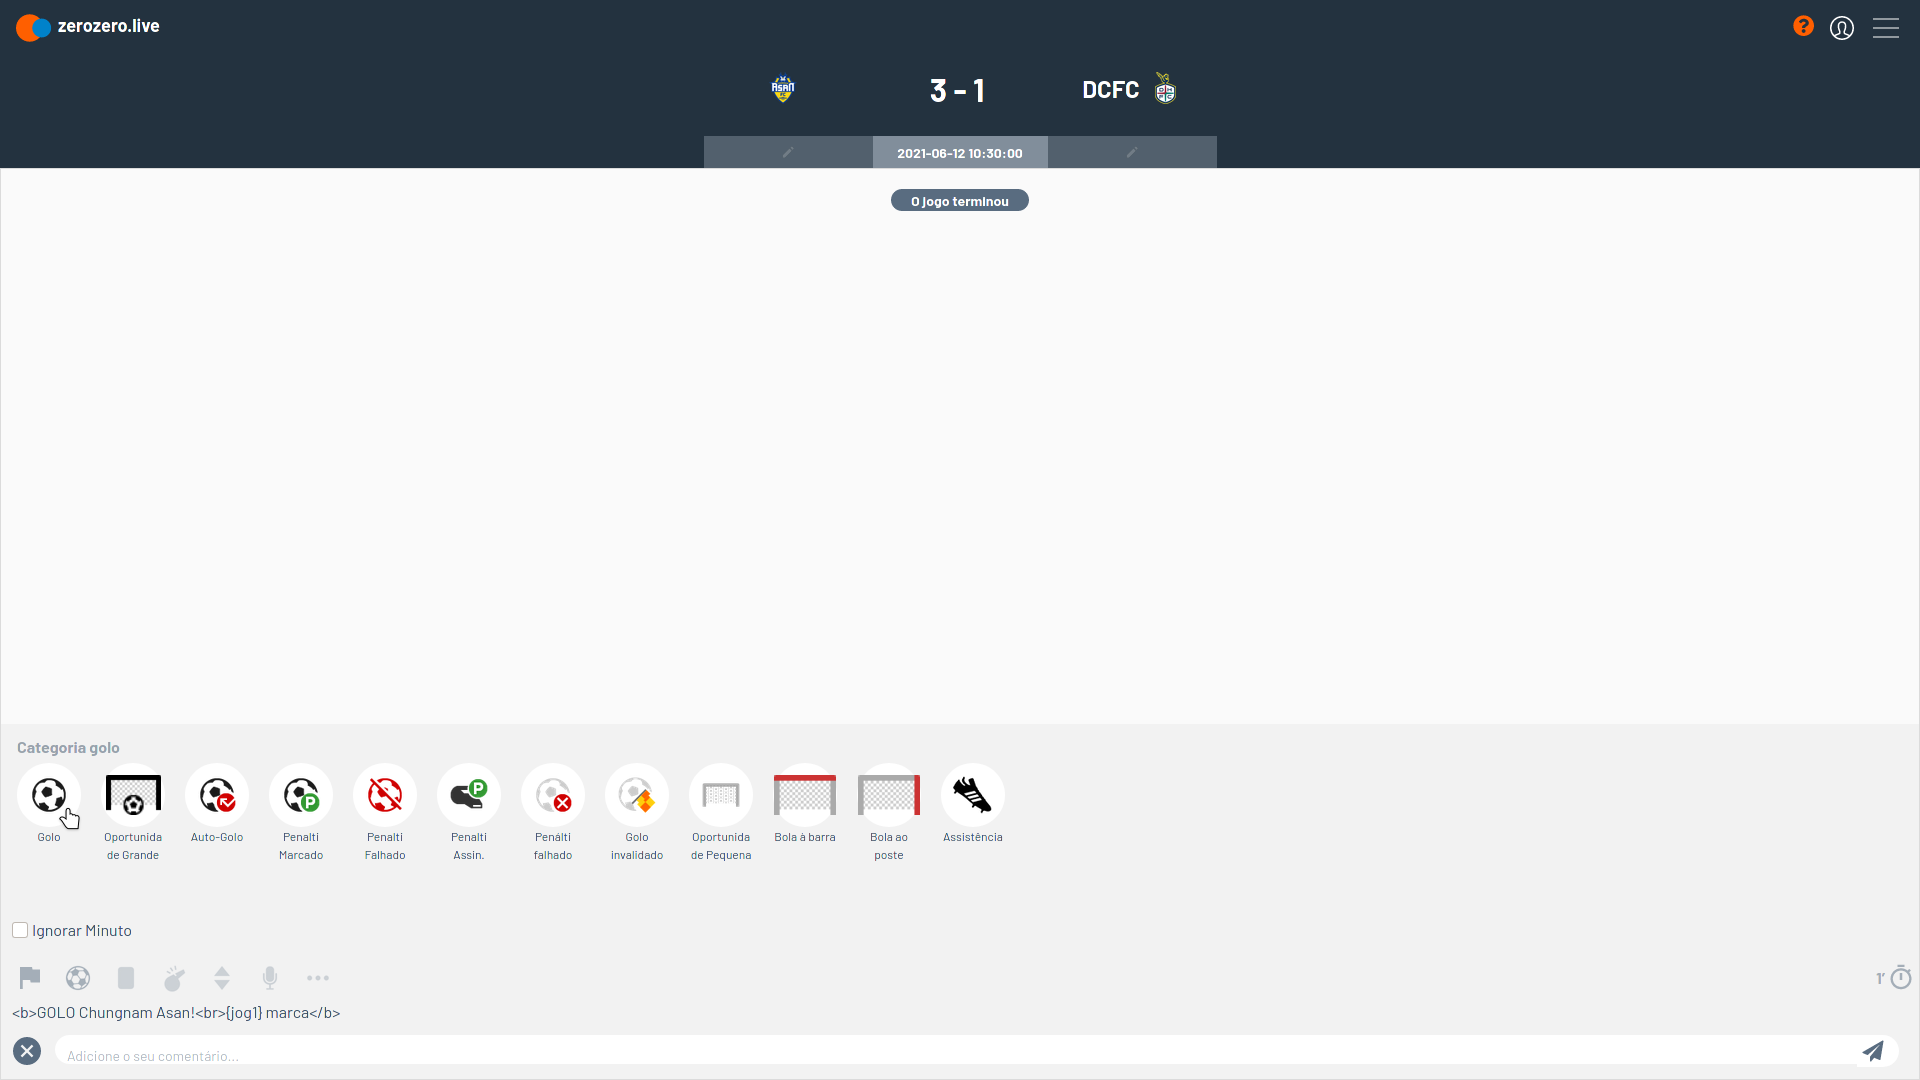
\includegraphics[width=\textwidth]{zerozerolive-event-select.png}
        \caption{Event selection}
        \label{fig:zerozerolive-event-select}
    \end{center}
\end{figure}

\begin{figure}[h]
    \begin{center}
        \leavevmode
        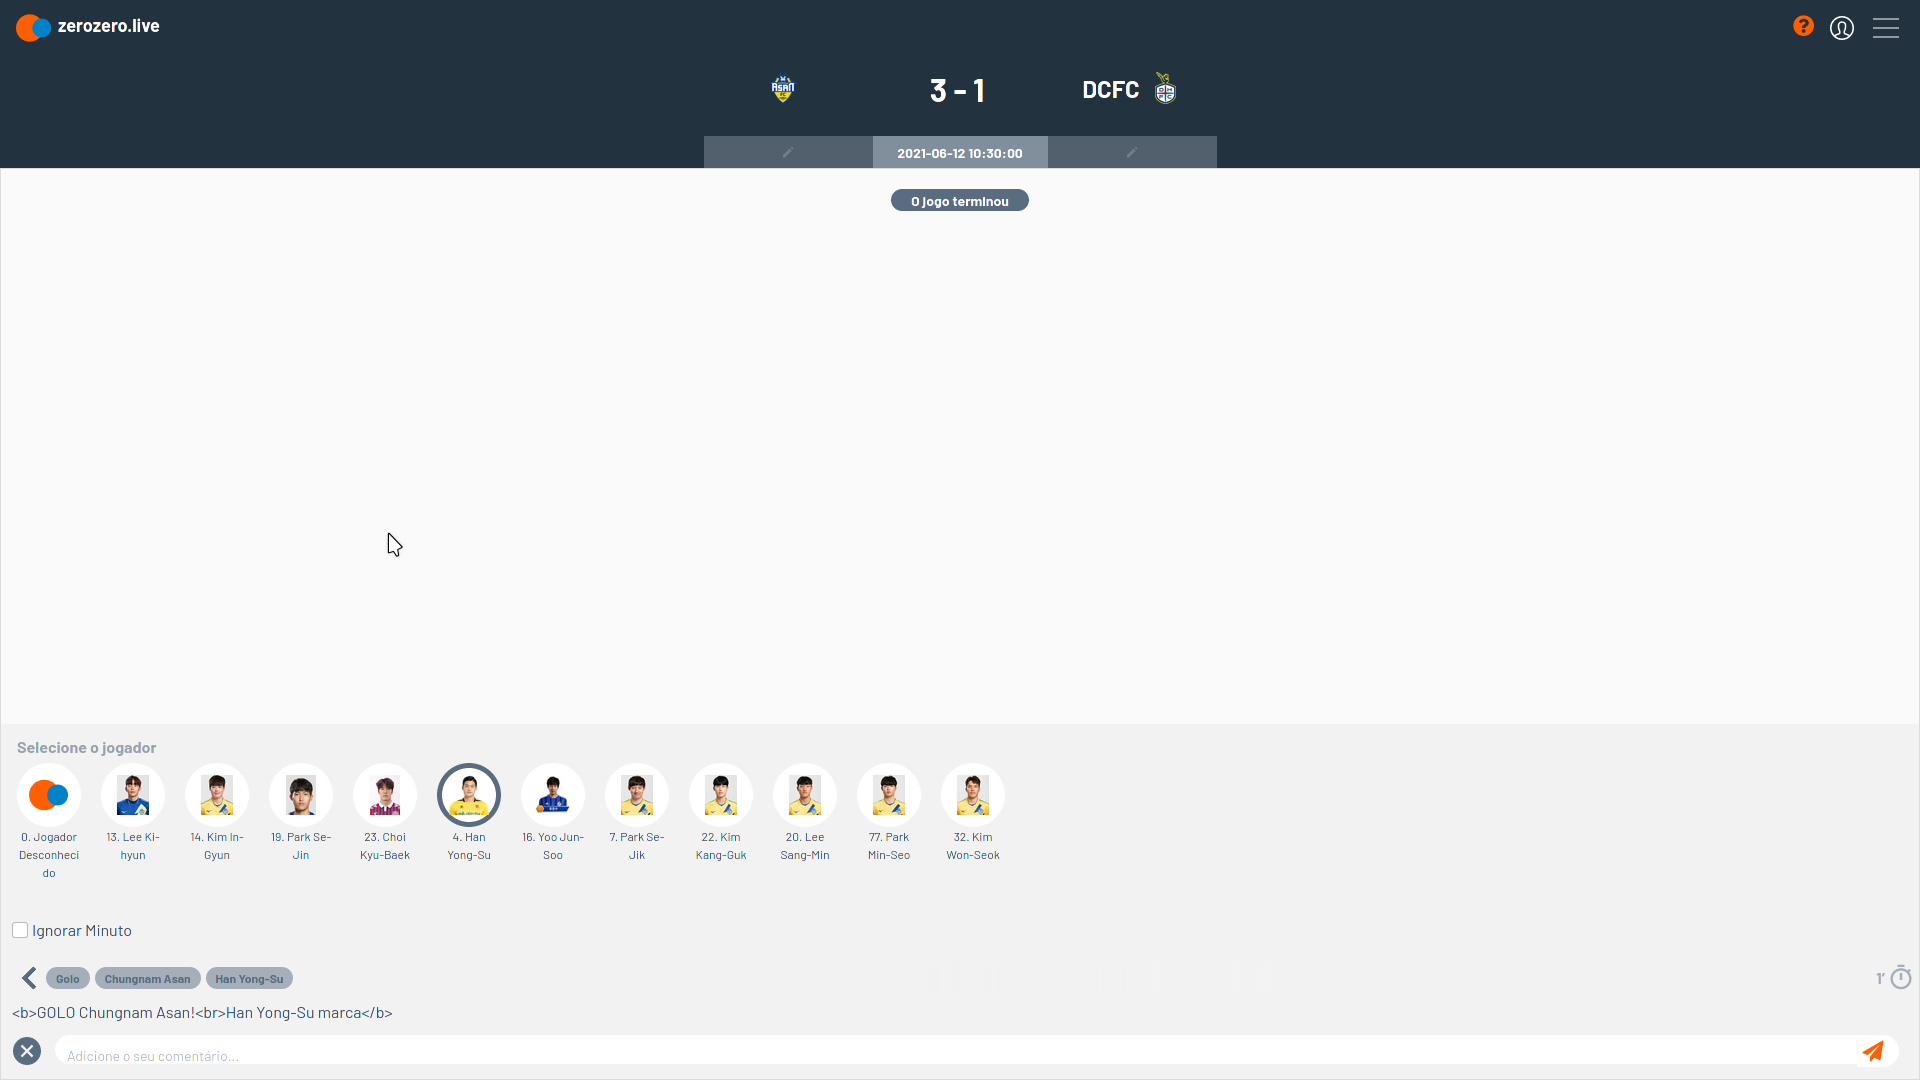
\includegraphics[width=\textwidth]{zerozerolive-event-player-select.png}
        \caption{Event's player selection}
        \label{fig:zerozerolive-event-player-select}
    \end{center}
\end{figure}

As was previously mentioned, a big part of this project is the synchronization with the ZeroZero API events. On startup, the application will check which event are on the API registry that are currently not on the ZeroZero Live database. If it finds any, it will try to synchronize them by inserting them in the local PouchDB database, and then replicating to the remote database. The complete algorithm is mentioned in more detail above, on Section~\ref{sec:api-sync}. 

%events interactions(insert, edit delete) (to local then remote)
Regarding the event operations, namely insert, edit, and delete, the process is similar to each of them. A document is pushed to the local database, which makes it show on the UI for the user. Then it is synchronized to the remote database which, due to the replication listener will make it show on other users' machines as well, as soon as it replicates to their local databases. It may happen that during these replications a conflict arises. In those cases, the conflict icon is shown on the event, and the user can resolve the conflict after clicking there and examining the solution candidates. Figure~\ref{fig:zerozerolive-conflict-resolution} shows the conflict resolution interface, where the user can select a \say{winner} event, or choose to keep all events in the match. The resolutions strategies were already discussed above, in Section~\ref{list:conflict-resolution-strategies-frontend}

\begin{figure}[h]
    \begin{center}
        \leavevmode
        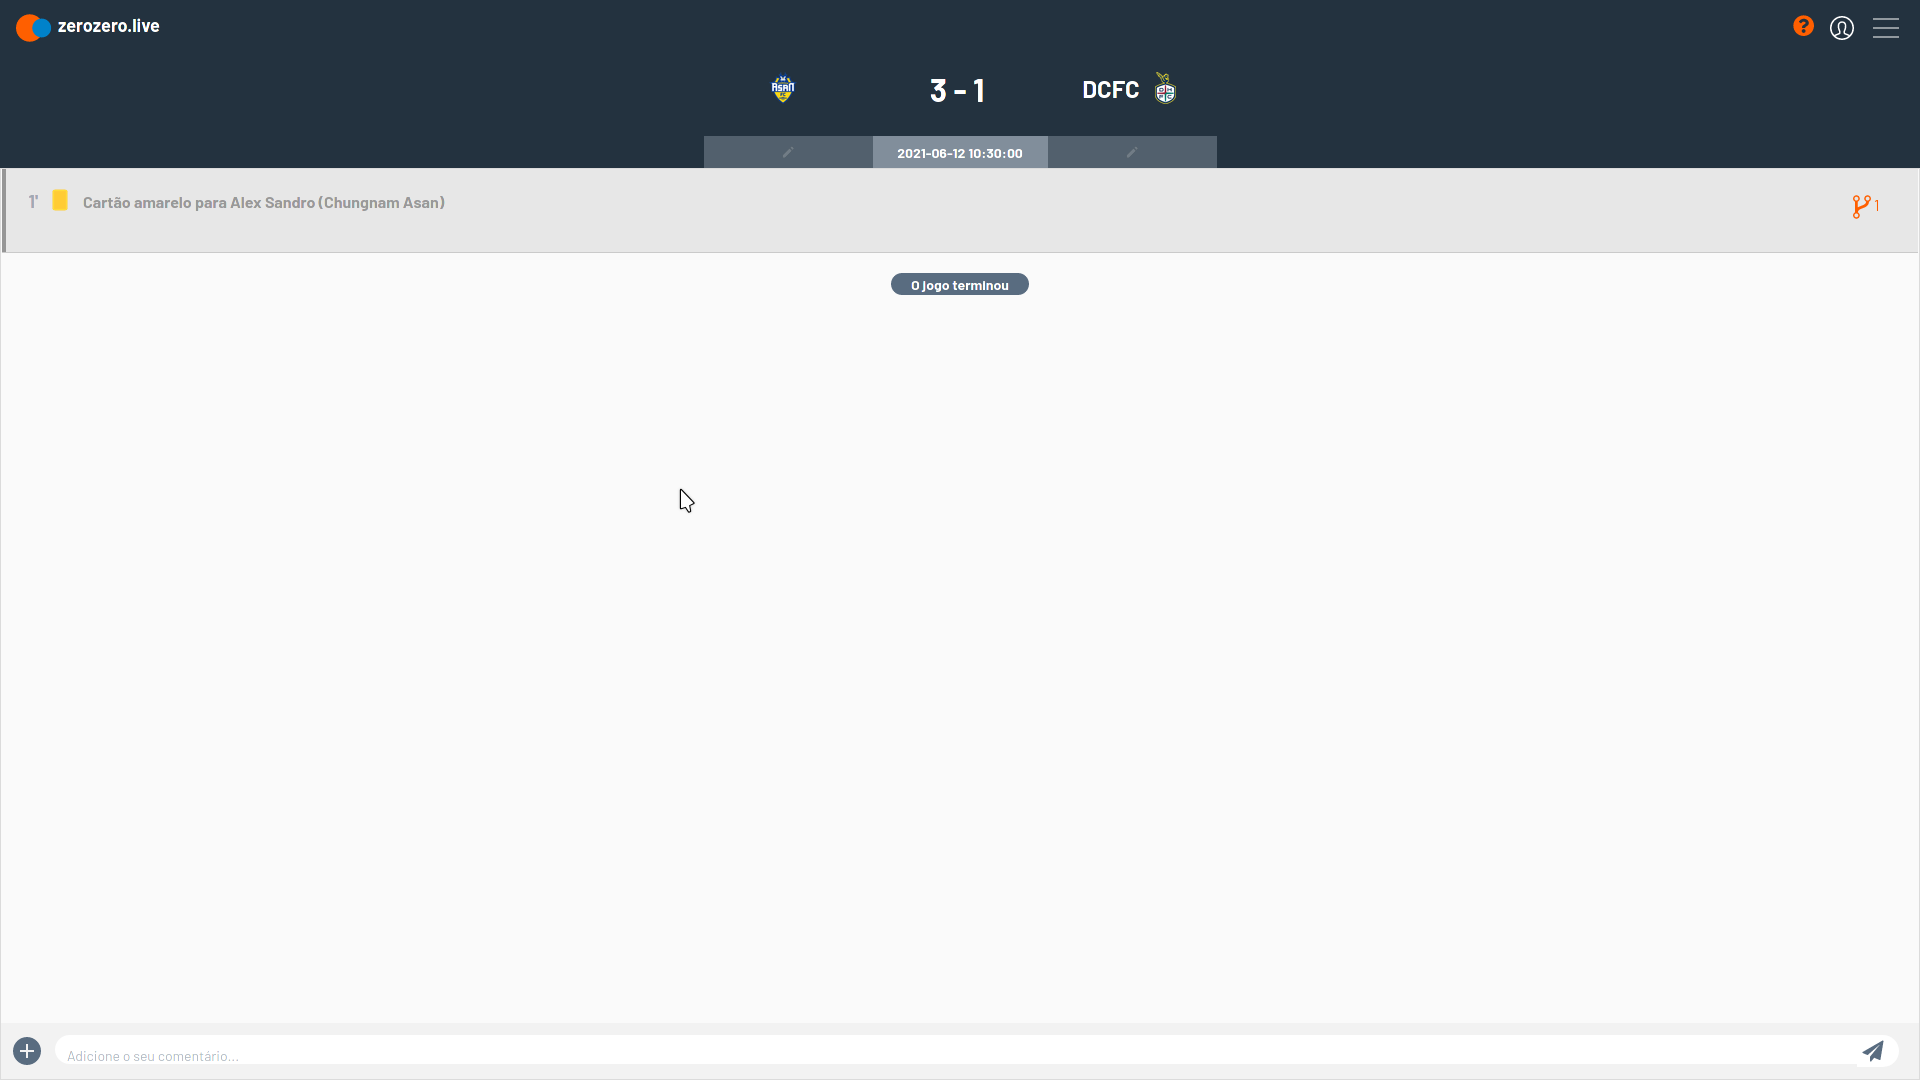
\includegraphics[width=\textwidth]{zerozerolive-conflict-event.png}
        \caption{Event with a conflict pending resolution}
        \label{fig:zerozerolive-conflict-event}
    \end{center}
\end{figure}

\begin{figure}[h]
    \begin{center}
        \leavevmode
        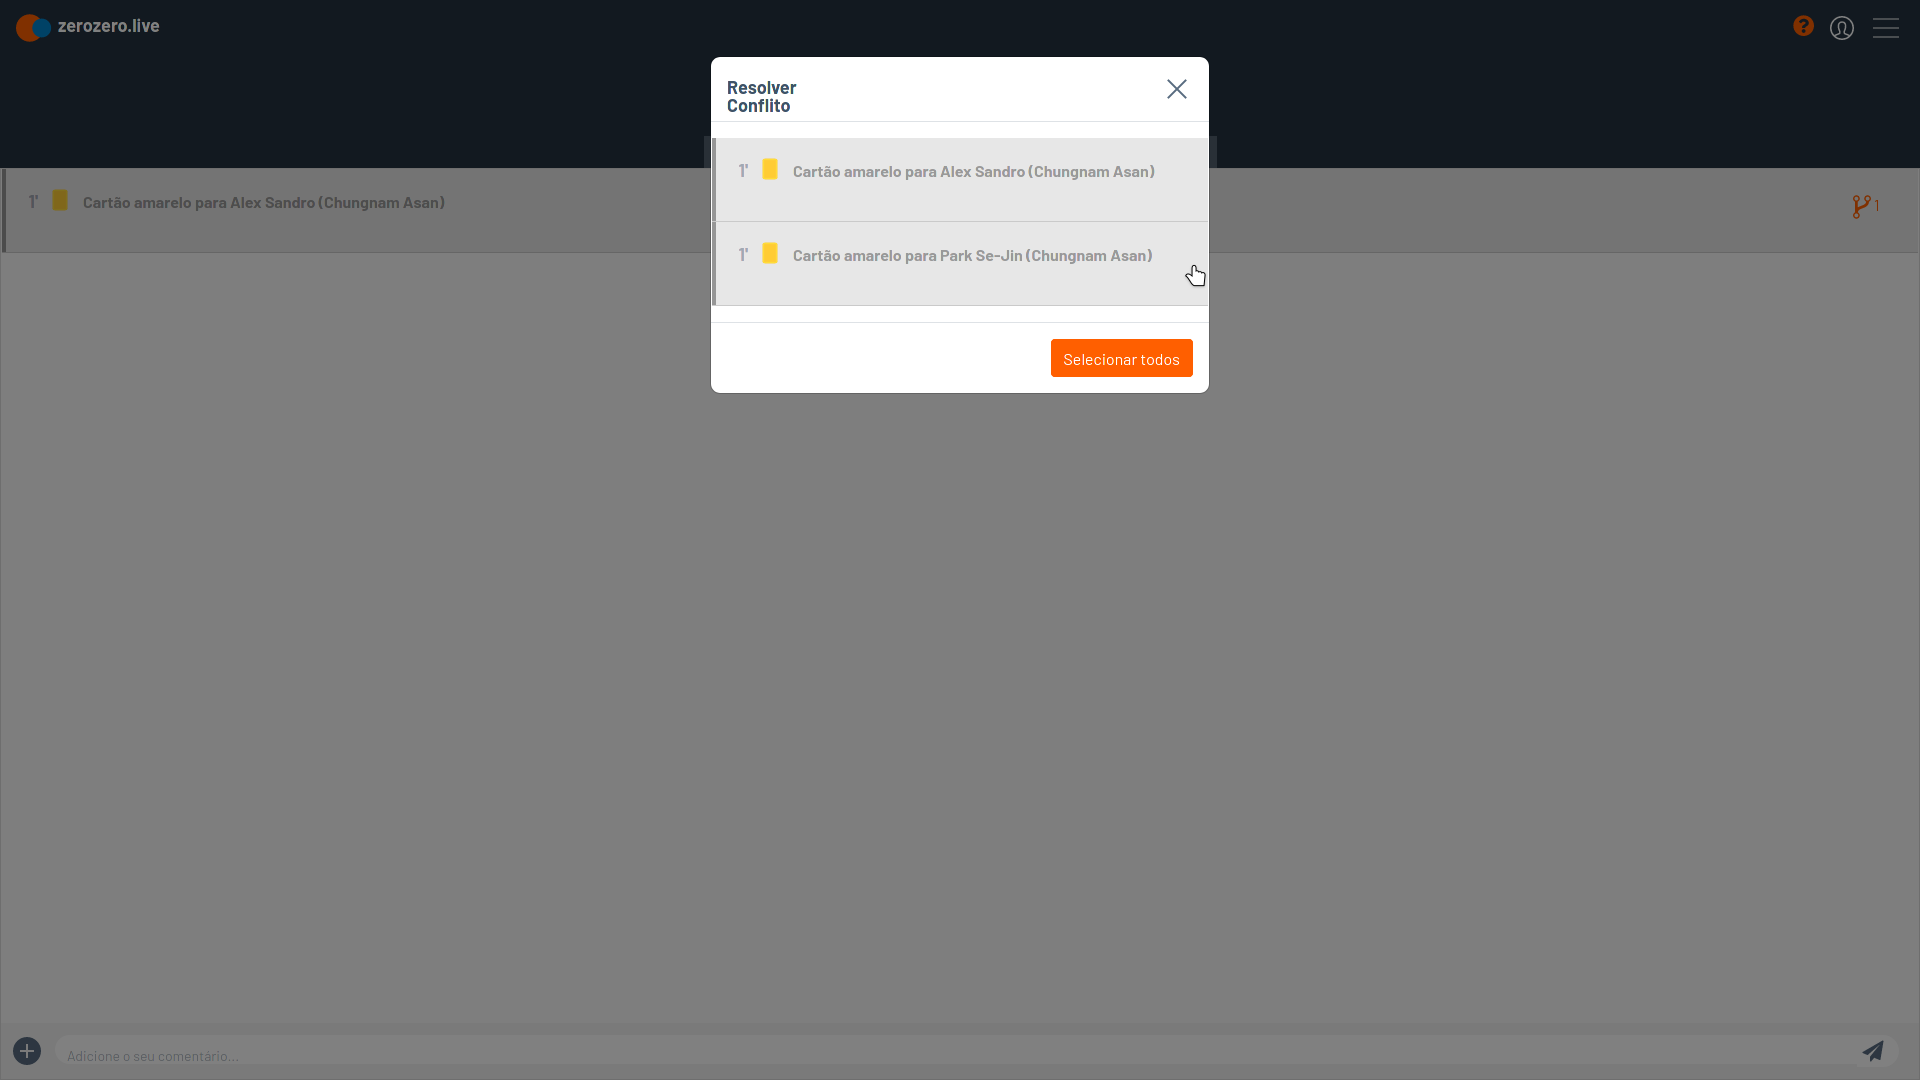
\includegraphics[width=\textwidth]{zerozerolive-conflict-resolution.png}
        \caption{Event conflict resolution interface}
        \label{fig:zerozerolive-conflict-resolution}
    \end{center}
\end{figure}

Figure~\ref{fig:insert_doc_seq_noconf} shows the sequence of operations when an event is inserted on the frontend (Browser), when there is no conflict. First the document is created on the local database, which is then replicated to the remote database. Once the remote database receives a document, it will emit events for any listener, including the clients and the conflict handler which, when receiving a document without conflicts, will try to synchronize it to the ZeroZero API, by inserting it in this case. As was previously mentioned, it will then update the document by setting its \say{insert} field to $false$. That change will once again be propagated to all listening clients.

In the case of conflicts, Figure~\ref{fig:insert_doc_seq_conf} shows that the sequence of operations is slightly different when the conflict handler receives the conflicting document. It will resolve it first, before trying to synchronize anything. One thing to note is that the UI will receive the conflicting event while it is being resolved. For the users, it is as if someone is resolving a conflict really fast, as they might see the conflict appear and quickly be resolved, since the changes are always replicated to all listening clients. After resolving the conflict and receiving the updated document back, the conflict handler will behave like the previous example and synchronize the documents accordingly.

\begin{figure}[h]
    \begin{center}
        \leavevmode
        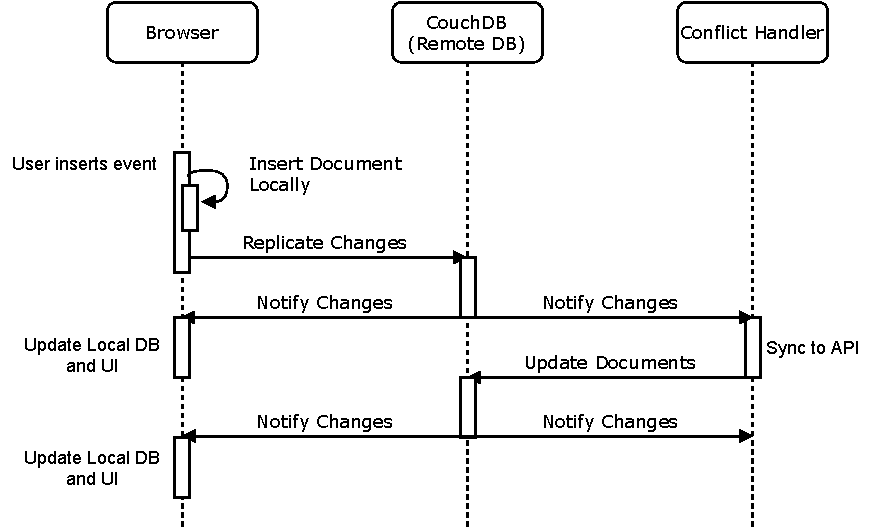
\includegraphics[width=\textwidth]{insert_doc_seq_noconf.pdf}
        \caption{Sequence diagram representing the flow when inserting an event without conflicts}
        \label{fig:insert_doc_seq_noconf}
    \end{center}
\end{figure}

\begin{figure}[h]
    \begin{center}
        \leavevmode
        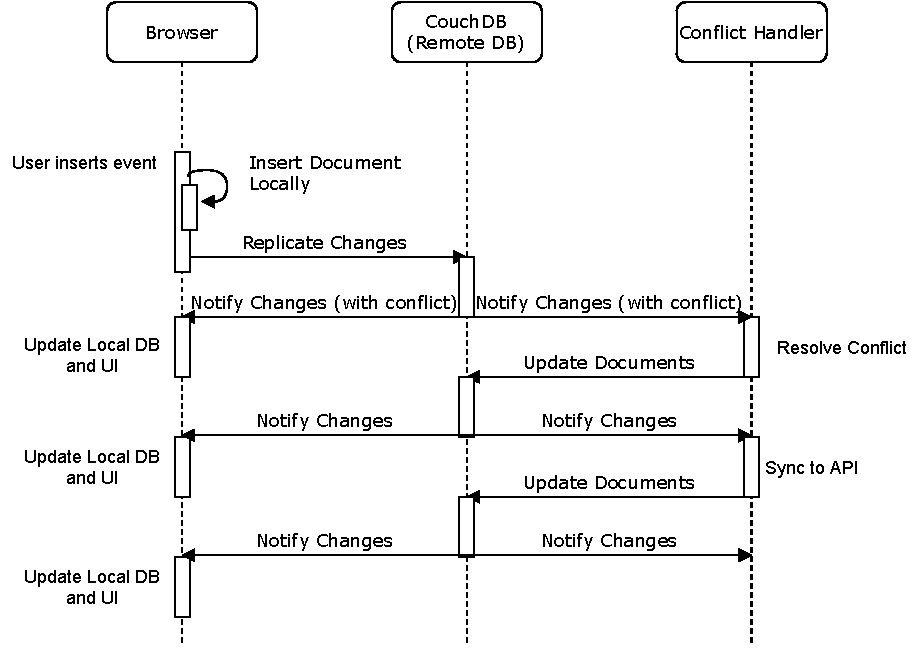
\includegraphics[width=\textwidth]{insert_doc_seq_conf.pdf}
        \caption{Sequence diagram representing the flow when inserting an event with conflicts}
        \label{fig:insert_doc_seq_conf}
    \end{center}
\end{figure}

\section{Time synchronization}

An important part of a real-time application is the time synchronization between users and the server itself. In this application this is done by clients fetching the game start time from the ZeroZero API, and calculating the game time locally. It has a big problem, as we eventually found out, since clients may not be synchronized with the server themselves. A similar scenario happened inside ZOS, while we were testing the application. Some of the computers in the office had their clocks offset by a couple minutes in relation to the server serving the application. This resulted in a shift on the match minute they were seeing. This happened since the match clock is calculated based on the start time specified on the server and the current client time. In order to fix this problem, and any similar issues that can happen for users in different timezones, an offset correction value was added. The clients now send their local time when requesting the match information, and the server will return an offset in relation to its own time, which clients can use to fix the clock calculation, and make sure all are synchronized, independently of their local times.

\section{Summary}
In summary, a microservice architecture was used to build the application to solve the problem defined in Chapter~\ref{chap:problem}. In order to organize the deployment and treat the whole system as a unit instead of managing all the microservices individually, Docker Compose was used. In order to allow multiple services to be reached through the same domain, a reverse proxy service was developed, which routed the requests to the different services based on the used endpoint. In order to deal with conflicts detection and resolution, CouchDB was used, which has these features built-in to its design, while allowing an easy replication and offline usage, by using its local counterpart, PouchDB. Additionally, a reputation HTTP server was developed to handle the user reputation, which takes into account the users' reputations in order to have a dynamic influence on each others' inputs, as well as a decay of reputation over time, if users become inactive. All of these features were visible to the user through the web application frontend, which allowed for match coverage, by selecting the teams' rosters and events inputting, describing what is happening in real time. It further allows for manual conflict resolution when the automatic resolver chooses not to resolve the conflict.